\documentclass[11pt]{article}

% The four macros of the header standard; tools/zenodo/publish_revision.py patches them when it reserves the DOI.
\newcommand{\doctype}{Preprint}
\newcommand{\docversion}{v1.00.000}
\newcommand{\docdate}{8 November 2026}
\newcommand{\versiondoi}{10.5281/zenodo.24053215}
\newcommand{\conceptdoi}{10.5281/zenodo.24053214}
\newcommand{\docidentity}{CAOS\_Contraste, the validation of the risk models of a bank}

% The packages and conventions every Contraste manuscript shares (CAOS_MANAGE conventions/manuscript-content-bar.md
% section 2). A document sets its class, the four header macros and \docidentity, then % The packages and conventions every Contraste manuscript shares (CAOS_MANAGE conventions/manuscript-content-bar.md
% section 2). A document sets its class, the four header macros and \docidentity, then % The packages and conventions every Contraste manuscript shares (CAOS_MANAGE conventions/manuscript-content-bar.md
% section 2). A document sets its class, the four header macros and \docidentity, then \input{../_shared/preamble}.
\usepackage[T1]{fontenc}
\usepackage[utf8]{inputenc}
\usepackage{lmodern}
\usepackage{microtype}
\usepackage[a4paper,margin=2.5cm]{geometry}
\usepackage{amsmath,amssymb,amsthm,mathtools,bm}
\usepackage{graphicx}
\usepackage{booktabs,longtable,tabularx,array,multirow}
\usepackage{siunitx}
\usepackage{algorithm}
\usepackage{algpseudocode}
\usepackage{caption,subcaption}
\usepackage{xcolor}
\usepackage[numbers,sort&compress]{natbib}
\usepackage[hidelinks]{hyperref}
\usepackage{cleveref}
\usepackage{orcidlink}

\sisetup{group-separator={,},group-minimum-digits=4,detect-all}
\graphicspath{{figures/}{../figures/}}
\captionsetup{font=small,labelfont=bf}
\setlength{\LTcapwidth}{\textwidth}

% Theorem environments for the Theory sections of the manuscripts.
\newtheorem{proposition}{Proposition}
\newtheorem{lemma}{Lemma}
\newtheorem{corollary}{Corollary}
\theoremstyle{definition}
\newtheorem{definition}{Definition}
\newtheorem{assumption}{Assumption}
\theoremstyle{remark}
\newtheorem{remark}{Remark}

% Notation shared by the documents (each defines it again in its notation table).
\newcommand{\E}{\mathbb{E}}
\newcommand{\Prob}{\mathbb{P}}
\newcommand{\Var}{\operatorname{Var}}
\newcommand{\Cov}{\operatorname{Cov}}
\newcommand{\VaR}{\operatorname{VaR}}
\newcommand{\ES}{\operatorname{ES}}
\newcommand{\PD}{\mathrm{PD}}
\newcommand{\LGD}{\mathrm{LGD}}
\newcommand{\EAD}{\mathrm{EAD}}
\newcommand{\ECL}{\mathrm{ECL}}
\newcommand{\indic}{\mathbf{1}}
\newcommand{\R}{\mathbb{R}}
\newcommand{\dd}{\,\mathrm{d}}

% The page-1 header block (CAOS_MANAGE conventions/manuscript-header-standard.md). The document defines \doctype,
% \docversion, \docdate, \versiondoi, \conceptdoi and \docidentity before this file; the publishing tool patches the four
% macros of the standard when it reserves the version DOI.
\newcommand{\docrepo}{github.com/fsantibanezleal/CAOS\_Contraste}
\newcommand{\headerblock}{%
\begin{center}
\fbox{\parbox{0.94\textwidth}{\small\raggedright
\textbf{\doctype} \quad$\cdot$\quad \docversion, \docdate \quad$\cdot$\quad Licence CC BY 4.0\\[2pt]
CAOS open-research programme \quad$\cdot$\quad \docidentity\\[2pt]
Version DOI \href{https://doi.org/\versiondoi}{\texttt{\versiondoi}} \quad$\cdot$\quad
concept DOI (always latest) \href{https://doi.org/\conceptdoi}{\texttt{\conceptdoi}}\\[2pt]
Not peer reviewed. Source code, data and computational records: \href{https://\docrepo}{\texttt{\docrepo}}
}}
\end{center}
\vspace{4pt}}
.
\usepackage[T1]{fontenc}
\usepackage[utf8]{inputenc}
\usepackage{lmodern}
\usepackage{microtype}
\usepackage[a4paper,margin=2.5cm]{geometry}
\usepackage{amsmath,amssymb,amsthm,mathtools,bm}
\usepackage{graphicx}
\usepackage{booktabs,longtable,tabularx,array,multirow}
\usepackage{siunitx}
\usepackage{algorithm}
\usepackage{algpseudocode}
\usepackage{caption,subcaption}
\usepackage{xcolor}
\usepackage[numbers,sort&compress]{natbib}
\usepackage[hidelinks]{hyperref}
\usepackage{cleveref}
\usepackage{orcidlink}

\sisetup{group-separator={,},group-minimum-digits=4,detect-all}
\graphicspath{{figures/}{../figures/}}
\captionsetup{font=small,labelfont=bf}
\setlength{\LTcapwidth}{\textwidth}

% Theorem environments for the Theory sections of the manuscripts.
\newtheorem{proposition}{Proposition}
\newtheorem{lemma}{Lemma}
\newtheorem{corollary}{Corollary}
\theoremstyle{definition}
\newtheorem{definition}{Definition}
\newtheorem{assumption}{Assumption}
\theoremstyle{remark}
\newtheorem{remark}{Remark}

% Notation shared by the documents (each defines it again in its notation table).
\newcommand{\E}{\mathbb{E}}
\newcommand{\Prob}{\mathbb{P}}
\newcommand{\Var}{\operatorname{Var}}
\newcommand{\Cov}{\operatorname{Cov}}
\newcommand{\VaR}{\operatorname{VaR}}
\newcommand{\ES}{\operatorname{ES}}
\newcommand{\PD}{\mathrm{PD}}
\newcommand{\LGD}{\mathrm{LGD}}
\newcommand{\EAD}{\mathrm{EAD}}
\newcommand{\ECL}{\mathrm{ECL}}
\newcommand{\indic}{\mathbf{1}}
\newcommand{\R}{\mathbb{R}}
\newcommand{\dd}{\,\mathrm{d}}

% The page-1 header block (CAOS_MANAGE conventions/manuscript-header-standard.md). The document defines \doctype,
% \docversion, \docdate, \versiondoi, \conceptdoi and \docidentity before this file; the publishing tool patches the four
% macros of the standard when it reserves the version DOI.
\newcommand{\docrepo}{github.com/fsantibanezleal/CAOS\_Contraste}
\newcommand{\headerblock}{%
\begin{center}
\fbox{\parbox{0.94\textwidth}{\small\raggedright
\textbf{\doctype} \quad$\cdot$\quad \docversion, \docdate \quad$\cdot$\quad Licence CC BY 4.0\\[2pt]
CAOS open-research programme \quad$\cdot$\quad \docidentity\\[2pt]
Version DOI \href{https://doi.org/\versiondoi}{\texttt{\versiondoi}} \quad$\cdot$\quad
concept DOI (always latest) \href{https://doi.org/\conceptdoi}{\texttt{\conceptdoi}}\\[2pt]
Not peer reviewed. Source code, data and computational records: \href{https://\docrepo}{\texttt{\docrepo}}
}}
\end{center}
\vspace{4pt}}
.
\usepackage[T1]{fontenc}
\usepackage[utf8]{inputenc}
\usepackage{lmodern}
\usepackage{microtype}
\usepackage[a4paper,margin=2.5cm]{geometry}
\usepackage{amsmath,amssymb,amsthm,mathtools,bm}
\usepackage{graphicx}
\usepackage{booktabs,longtable,tabularx,array,multirow}
\usepackage{siunitx}
\usepackage{algorithm}
\usepackage{algpseudocode}
\usepackage{caption,subcaption}
\usepackage{xcolor}
\usepackage[numbers,sort&compress]{natbib}
\usepackage[hidelinks]{hyperref}
\usepackage{cleveref}
\usepackage{orcidlink}

\sisetup{group-separator={,},group-minimum-digits=4,detect-all}
\graphicspath{{figures/}{../figures/}}
\captionsetup{font=small,labelfont=bf}
\setlength{\LTcapwidth}{\textwidth}

% Theorem environments for the Theory sections of the manuscripts.
\newtheorem{proposition}{Proposition}
\newtheorem{lemma}{Lemma}
\newtheorem{corollary}{Corollary}
\theoremstyle{definition}
\newtheorem{definition}{Definition}
\newtheorem{assumption}{Assumption}
\theoremstyle{remark}
\newtheorem{remark}{Remark}

% Notation shared by the documents (each defines it again in its notation table).
\newcommand{\E}{\mathbb{E}}
\newcommand{\Prob}{\mathbb{P}}
\newcommand{\Var}{\operatorname{Var}}
\newcommand{\Cov}{\operatorname{Cov}}
\newcommand{\VaR}{\operatorname{VaR}}
\newcommand{\ES}{\operatorname{ES}}
\newcommand{\PD}{\mathrm{PD}}
\newcommand{\LGD}{\mathrm{LGD}}
\newcommand{\EAD}{\mathrm{EAD}}
\newcommand{\ECL}{\mathrm{ECL}}
\newcommand{\indic}{\mathbf{1}}
\newcommand{\R}{\mathbb{R}}
\newcommand{\dd}{\,\mathrm{d}}

% The page-1 header block (CAOS_MANAGE conventions/manuscript-header-standard.md). The document defines \doctype,
% \docversion, \docdate, \versiondoi, \conceptdoi and \docidentity before this file; the publishing tool patches the four
% macros of the standard when it reserves the version DOI.
\newcommand{\docrepo}{github.com/fsantibanezleal/CAOS\_Contraste}
\newcommand{\headerblock}{%
\begin{center}
\fbox{\parbox{0.94\textwidth}{\small\raggedright
\textbf{\doctype} \quad$\cdot$\quad \docversion, \docdate \quad$\cdot$\quad Licence CC BY 4.0\\[2pt]
CAOS open-research programme \quad$\cdot$\quad \docidentity\\[2pt]
Version DOI \href{https://doi.org/\versiondoi}{\texttt{\versiondoi}} \quad$\cdot$\quad
concept DOI (always latest) \href{https://doi.org/\conceptdoi}{\texttt{\conceptdoi}}\\[2pt]
Not peer reviewed. Source code, data and computational records: \href{https://\docrepo}{\texttt{\docrepo}}
}}
\end{center}
\vspace{4pt}}

% Generated by tables/make_tables.py: the numbers the prose quotes. Do not edit.
\newcommand{\valDate}{2026-09-03}
\newcommand{\ufValue}{40{,}877.73}
\newcommand{\tierOne}{824{,}214}
\newcommand{\clpAssets}{4{,}988{,}540}
\newcommand{\clpLiabs}{4{,}411{,}591}
\newcommand{\urAssetsUf}{66}
\newcommand{\urLiabsUf}{60}
\newcommand{\nItemsClp}{12}
\newcommand{\nItemsUr}{5}
\newcommand{\rmseClp}{0.50}
\newcommand{\shortClp}{4.50}
\newcommand{\longClp}{5.91}
\newcommand{\minClp}{4.49}
\newcommand{\maxClp}{5.91}
\newcommand{\nTenorsClp}{4}
\newcommand{\rmseUr}{0.41}
\newcommand{\shortUr}{1.20}
\newcommand{\longUr}{2.84}
\newcommand{\minUr}{1.20}
\newcommand{\maxUr}{2.84}
\newcommand{\nTenorsUr}{4}
\newcommand{\spreadFive}{318}
\newcommand{\spreadLast}{307}
\newcommand{\spreadFirst}{329}
\newcommand{\dfRatioFive}{0.840}
\newcommand{\dfRatioTen}{0.741}
\newcommand{\dfRatioLast}{0.464}
\newcommand{\sizeRatio}{1.50}
\newcommand{\weightFive}{1.26}
\newcommand{\weightTen}{1.11}
\newcommand{\weightLast}{0.70}
\newcommand{\tStarLo}{12.5}
\newcommand{\tStarHi}{17.5}
\newcommand{\repMaxDev}{0}
\newcommand{\repSandChecked}{384}
\newcommand{\repSandViol}{0}
\newcommand{\repAnnexEveLng}{93{,}816}
\newcommand{\repAnnexNiiLng}{11{,}213}
\newcommand{\repSingleEveLng}{84{,}710}
\newcommand{\repSingleNiiLng}{1{,}648}
\newcommand{\repPosEveLng}{94{,}721}
\newcommand{\repPosNiiLng}{8{,}415}
\newcommand{\repGapNiiLng}{1{,}648}
\newcommand{\repGapEveLng}{98{,}166}
\newcommand{\repChargeLng}{6{,}182}
\newcommand{\repMaxPairLng}{5{,}032}
\newcommand{\repChargeShareLng}{55.1}
\newcommand{\repRatioNiiLng}{6.8}
\newcommand{\repEveShortLng}{9.7}
\newcommand{\repNuLng}{30}
\newcommand{\repPnUrLng}{247{,}264}
\newcommand{\repMarginLng}{261{,}022}
\newcommand{\repNiiTLng}{1.36}
\newcommand{\repEveTLng}{11.4}
\newcommand{\repEveTSingleLng}{10.3}
\newcommand{\repEveTPosLng}{11.5}
\newcommand{\repFloorDistLng}{20.48}
\newcommand{\repAssetUnderLng}{16.5}
\newcommand{\repLiabUnderLng}{11.0}
\newcommand{\repAnnexEveSht}{79{,}643}
\newcommand{\repAnnexNiiSht}{11{,}067}
\newcommand{\repSingleEveSht}{64{,}213}
\newcommand{\repSingleNiiSht}{1{,}356}
\newcommand{\repPosEveSht}{79{,}643}
\newcommand{\repPosNiiSht}{8{,}415}
\newcommand{\repGapNiiSht}{1{,}356}
\newcommand{\repGapEveSht}{73{,}544}
\newcommand{\repChargeSht}{6{,}182}
\newcommand{\repMaxPairSht}{4{,}885}
\newcommand{\repChargeShareSht}{55.9}
\newcommand{\repRatioNiiSht}{8.2}
\newcommand{\repEveShortSht}{19.4}
\newcommand{\repNuSht}{30}
\newcommand{\repPnUrSht}{247{,}264}
\newcommand{\repMarginSht}{274{,}664}
\newcommand{\repNiiTSht}{1.34}
\newcommand{\repEveTSht}{9.7}
\newcommand{\repEveTSingleSht}{7.8}
\newcommand{\repEveTPosSht}{9.7}
\newcommand{\repFloorDistSht}{20.48}
\newcommand{\repAssetUnderSht}{16.5}
\newcommand{\repLiabUnderSht}{12.1}
\newcommand{\repAnnexEveCpi}{93{,}816}
\newcommand{\repAnnexNiiCpi}{11{,}213}
\newcommand{\repSingleEveCpi}{84{,}710}
\newcommand{\repSingleNiiCpi}{1{,}648}
\newcommand{\repPosEveCpi}{94{,}721}
\newcommand{\repPosNiiCpi}{8{,}415}
\newcommand{\repGapNiiCpi}{1{,}648}
\newcommand{\repGapEveCpi}{98{,}166}
\newcommand{\repChargeCpi}{6{,}182}
\newcommand{\repMaxPairCpi}{5{,}032}
\newcommand{\repChargeShareCpi}{55.1}
\newcommand{\repRatioNiiCpi}{6.8}
\newcommand{\repEveShortCpi}{9.7}
\newcommand{\repNuCpi}{30}
\newcommand{\repPnUrCpi}{247{,}264}
\newcommand{\repMarginCpi}{261{,}022}
\newcommand{\repNiiTCpi}{1.36}
\newcommand{\repEveTCpi}{11.4}
\newcommand{\repEveTSingleCpi}{10.3}
\newcommand{\repEveTPosCpi}{11.5}
\newcommand{\repFloorDistCpi}{20.48}
\newcommand{\repAssetUnderCpi}{16.5}
\newcommand{\repLiabUnderCpi}{11.0}
\newcommand{\repAnnexEveStp}{140{,}645}
\newcommand{\repAnnexNiiStp}{6{,}783}
\newcommand{\repSingleEveStp}{129{,}432}
\newcommand{\repSingleNiiStp}{3{,}091}
\newcommand{\repPosEveStp}{140{,}645}
\newcommand{\repPosNiiStp}{8{,}415}
\newcommand{\repGapNiiStp}{3{,}091}
\newcommand{\repGapEveStp}{162{,}183}
\newcommand{\repChargeStp}{1{,}030}
\newcommand{\repMaxPairStp}{5{,}753}
\newcommand{\repChargeShareStp}{15.2}
\newcommand{\repRatioNiiStp}{2.2}
\newcommand{\repEveShortStp}{8.0}
\newcommand{\repNuStp}{5}
\newcommand{\repPnUrStp}{41{,}211}
\newcommand{\repMarginStp}{278{,}048}
\newcommand{\repNiiTStp}{0.82}
\newcommand{\repEveTStp}{17.1}
\newcommand{\repEveTSingleStp}{15.7}
\newcommand{\repEveTPosStp}{17.1}
\newcommand{\repFloorDistStp}{20.48}
\newcommand{\repAssetUnderStp}{16.5}
\newcommand{\repLiabUnderStp}{11.5}
\newcommand{\repAnnexEveOff}{81{,}173}
\newcommand{\repAnnexNiiOff}{11{,}016}
\newcommand{\repSingleEveOff}{59{,}422}
\newcommand{\repSingleNiiOff}{1{,}254}
\newcommand{\repPosEveOff}{94{,}721}
\newcommand{\repPosNiiOff}{8{,}415}
\newcommand{\repGapNiiOff}{1{,}254}
\newcommand{\repGapEveOff}{66{,}893}
\newcommand{\repChargeOff}{6{,}182}
\newcommand{\repMaxPairOff}{4{,}834}
\newcommand{\repChargeShareOff}{56.1}
\newcommand{\repRatioNiiOff}{8.8}
\newcommand{\repEveShortOff}{26.8}
\newcommand{\repNuOff}{30}
\newcommand{\repPnUrOff}{247{,}264}
\newcommand{\repMarginOff}{258{,}182}
\newcommand{\repNiiTOff}{1.34}
\newcommand{\repEveTOff}{9.8}
\newcommand{\repEveTSingleOff}{7.2}
\newcommand{\repEveTPosOff}{11.5}
\newcommand{\repFloorDistOff}{20.48}
\newcommand{\repAssetUnderOff}{16.5}
\newcommand{\repLiabUnderOff}{11.0}
\newcommand{\repAnnexEveFlr}{60{,}764}
\newcommand{\repAnnexNiiFlr}{6{,}606}
\newcommand{\repSingleEveFlr}{49{,}837}
\newcommand{\repSingleNiiFlr}{4{,}653}
\newcommand{\repPosEveFlr}{60{,}764}
\newcommand{\repPosNiiFlr}{6{,}497}
\newcommand{\repGapNiiFlr}{4{,}653}
\newcommand{\repGapEveFlr}{57{,}279}
\newcommand{\repChargeFlr}{1{,}030}
\newcommand{\repMaxPairFlr}{5{,}575}
\newcommand{\repChargeShareFlr}{15.6}
\newcommand{\repRatioNiiFlr}{1.4}
\newcommand{\repEveShortFlr}{18.0}
\newcommand{\repNuFlr}{5}
\newcommand{\repPnUrFlr}{41{,}211}
\newcommand{\repMarginFlr}{261{,}583}
\newcommand{\repNiiTFlr}{0.80}
\newcommand{\repEveTFlr}{7.4}
\newcommand{\repEveTSingleFlr}{6.0}
\newcommand{\repEveTPosFlr}{7.4}
\newcommand{\repFloorDistFlr}{20.48}
\newcommand{\repAssetUnderFlr}{14.8}
\newcommand{\repLiabUnderFlr}{11.7}
\newcommand{\repCpiEffect}{6{,}182}
\newcommand{\repRatioLo}{6.8}
\newcommand{\repRatioHi}{8.8}
\newcommand{\repEveShortLo}{10}
\newcommand{\repEveShortHi}{27}
\newcommand{\repChargeOverTier}{0.75}
\newcommand{\repChargeShareLo}{55.1}
\newcommand{\repChargeShareHi}{56.1}
\newcommand{\floorBreakNu}{2.0}
\newcommand{\repFlagLng}{none}
\newcommand{\repFlagSht}{none}
\newcommand{\repFlagCpi}{none}
\newcommand{\repFlagStp}{eve-tier1}
\newcommand{\repFlagOff}{none}
\newcommand{\repFlagFlr}{none}
\newcommand{\mainSeeds}{30}
\newcommand{\mainSeconds}{18}
\newcommand{\repSeconds}{0.2}
\newcommand{\sweepSeconds}{3}
\newcommand{\floorsSeconds}{6}
\newcommand{\hOneChecked}{2{,}880}
\newcommand{\hOneViol}{0}
\newcommand{\hThreeChecked}{180}
\newcommand{\hThreeViol}{30}
\newcommand{\mainAnnexNiiLng}{11{,}907}
\newcommand{\mainAnnexNiiLngCi}{251}
\newcommand{\mainAnnexEveLng}{85{,}061}
\newcommand{\mainAnnexEveLngCi}{1{,}875}
\newcommand{\mainSingleNiiLng}{2{,}412}
\newcommand{\mainSingleNiiLngCi}{323}
\newcommand{\mainSingleEveLng}{80{,}186}
\newcommand{\mainSingleEveLngCi}{1{,}790}
\newcommand{\mainPosNiiLng}{9{,}039}
\newcommand{\mainPosNiiLngCi}{230}
\newcommand{\mainPosEveLng}{85{,}927}
\newcommand{\mainPosEveLngCi}{1{,}810}
\newcommand{\mainGapNiiLng}{2{,}412}
\newcommand{\mainGapNiiLngCi}{323}
\newcommand{\mainGapEveLng}{91{,}126}
\newcommand{\mainGapEveLngCi}{2{,}178}
\newcommand{\mainRatioNiiLng}{5.8}
\newcommand{\mainRatioNiiLngCi}{1.1}
\newcommand{\mainEveShortLng}{5.7}
\newcommand{\mainEveShortLngCi}{0.8}
\newcommand{\mainChargeShareLng}{52.1}
\newcommand{\mainChargeShareLngCi}{1.1}
\newcommand{\mainPosOverAnnexNiiLng}{0.76}
\newcommand{\mainPosOverAnnexEveLng}{1.010}
\newcommand{\mainGapOverAnnexEveLng}{1.07}
\newcommand{\mainSingleOverAnnexEveLng}{0.943}
\newcommand{\mainAnnexNiiTLng}{1.44}
\newcommand{\mainAnnexEveTLng}{10.3}
\newcommand{\mainShapEveCurveLng}{32{,}767}
\newcommand{\mainShapEveCurveLngCi}{956}
\newcommand{\mainShapEveSizesLng}{$-$28{,}757}
\newcommand{\mainShapEveSizesLngCi}{568}
\newcommand{\mainShapEveFloorLng}{0}
\newcommand{\mainShapEveFloorLngCi}{0}
\newcommand{\mainShapEvePairLng}{866}
\newcommand{\mainShapEvePairLngCi}{367}
\newcommand{\mainShapEveChargeLng}{0}
\newcommand{\mainShapEveChargeLngCi}{0}
\newcommand{\mainShapNiiCurveLng}{283}
\newcommand{\mainShapNiiCurveLngCi}{139}
\newcommand{\mainShapNiiSizesLng}{0}
\newcommand{\mainShapNiiSizesLngCi}{0}
\newcommand{\mainShapNiiFloorLng}{$-$172}
\newcommand{\mainShapNiiFloorLngCi}{101}
\newcommand{\mainShapNiiPairLng}{3{,}202}
\newcommand{\mainShapNiiPairLngCi}{99}
\newcommand{\mainShapNiiChargeLng}{6{,}182}
\newcommand{\mainShapNiiChargeLngCi}{0}
\newcommand{\mainLooEveCurveLng}{27{,}228}
\newcommand{\mainLooEveCurveLngCi}{800}
\newcommand{\mainLooEveSizesLng}{$-$34{,}296}
\newcommand{\mainLooEveSizesLngCi}{704}
\newcommand{\mainLooEveFloorLng}{0}
\newcommand{\mainLooEveFloorLngCi}{0}
\newcommand{\mainLooEvePairLng}{866}
\newcommand{\mainLooEvePairLngCi}{367}
\newcommand{\mainLooEveChargeLng}{0}
\newcommand{\mainLooEveChargeLngCi}{0}
\newcommand{\mainLooNiiCurveLng}{0}
\newcommand{\mainLooNiiCurveLngCi}{0}
\newcommand{\mainLooNiiSizesLng}{0}
\newcommand{\mainLooNiiSizesLngCi}{0}
\newcommand{\mainLooNiiFloorLng}{$-$122}
\newcommand{\mainLooNiiFloorLngCi}{134}
\newcommand{\mainLooNiiPairLng}{3{,}313}
\newcommand{\mainLooNiiPairLngCi}{125}
\newcommand{\mainLooNiiChargeLng}{6{,}182}
\newcommand{\mainLooNiiChargeLngCi}{0}
\newcommand{\mainAoiEveCurveLng}{38{,}306}
\newcommand{\mainAoiEveCurveLngCi}{1{,}112}
\newcommand{\mainAoiEveSizesLng}{$-$23{,}218}
\newcommand{\mainAoiEveSizesLngCi}{446}
\newcommand{\mainAoiEveFloorLng}{0}
\newcommand{\mainAoiEveFloorLngCi}{0}
\newcommand{\mainAoiEvePairLng}{866}
\newcommand{\mainAoiEvePairLngCi}{367}
\newcommand{\mainAoiEveChargeLng}{0}
\newcommand{\mainAoiEveChargeLngCi}{0}
\newcommand{\mainAoiNiiCurveLng}{787}
\newcommand{\mainAoiNiiCurveLngCi}{357}
\newcommand{\mainAoiNiiSizesLng}{0}
\newcommand{\mainAoiNiiSizesLngCi}{0}
\newcommand{\mainAoiNiiFloorLng}{0}
\newcommand{\mainAoiNiiFloorLngCi}{0}
\newcommand{\mainAoiNiiPairLng}{3{,}313}
\newcommand{\mainAoiNiiPairLngCi}{125}
\newcommand{\mainAoiNiiChargeLng}{6{,}182}
\newcommand{\mainAoiNiiChargeLngCi}{0}
\newcommand{\mainAnnexNiiSht}{11{,}772}
\newcommand{\mainAnnexNiiShtCi}{252}
\newcommand{\mainAnnexEveSht}{68{,}605}
\newcommand{\mainAnnexEveShtCi}{2{,}088}
\newcommand{\mainSingleNiiSht}{2{,}143}
\newcommand{\mainSingleNiiShtCi}{325}
\newcommand{\mainSingleEveSht}{58{,}057}
\newcommand{\mainSingleEveShtCi}{1{,}827}
\newcommand{\mainPosNiiSht}{9{,}039}
\newcommand{\mainPosNiiShtCi}{230}
\newcommand{\mainPosEveSht}{68{,}605}
\newcommand{\mainPosEveShtCi}{2{,}088}
\newcommand{\mainGapNiiSht}{2{,}143}
\newcommand{\mainGapNiiShtCi}{325}
\newcommand{\mainGapEveSht}{64{,}216}
\newcommand{\mainGapEveShtCi}{2{,}251}
\newcommand{\mainRatioNiiSht}{6.9}
\newcommand{\mainRatioNiiShtCi}{1.7}
\newcommand{\mainEveShortSht}{15.4}
\newcommand{\mainEveShortShtCi}{0.8}
\newcommand{\mainChargeShareSht}{52.7}
\newcommand{\mainChargeShareShtCi}{1.1}
\newcommand{\mainPosOverAnnexNiiSht}{0.77}
\newcommand{\mainPosOverAnnexEveSht}{1.000}
\newcommand{\mainGapOverAnnexEveSht}{0.94}
\newcommand{\mainSingleOverAnnexEveSht}{0.846}
\newcommand{\mainAnnexNiiTSht}{1.43}
\newcommand{\mainAnnexEveTSht}{8.3}
\newcommand{\mainShapEveCurveSht}{18{,}927}
\newcommand{\mainShapEveCurveShtCi}{1{,}029}
\newcommand{\mainShapEveSizesSht}{$-$8{,}379}
\newcommand{\mainShapEveSizesShtCi}{597}
\newcommand{\mainShapEveFloorSht}{0}
\newcommand{\mainShapEveFloorShtCi}{0}
\newcommand{\mainShapEvePairSht}{0}
\newcommand{\mainShapEvePairShtCi}{0}
\newcommand{\mainShapEveChargeSht}{0}
\newcommand{\mainShapEveChargeShtCi}{0}
\newcommand{\mainShapNiiCurveSht}{421}
\newcommand{\mainShapNiiCurveShtCi}{163}
\newcommand{\mainShapNiiSizesSht}{0}
\newcommand{\mainShapNiiSizesShtCi}{0}
\newcommand{\mainShapNiiFloorSht}{$-$257}
\newcommand{\mainShapNiiFloorShtCi}{122}
\newcommand{\mainShapNiiPairSht}{3{,}283}
\newcommand{\mainShapNiiPairShtCi}{97}
\newcommand{\mainShapNiiChargeSht}{6{,}182}
\newcommand{\mainShapNiiChargeShtCi}{0}
\newcommand{\mainLooEveCurveSht}{15{,}863}
\newcommand{\mainLooEveCurveShtCi}{860}
\newcommand{\mainLooEveSizesSht}{$-$11{,}443}
\newcommand{\mainLooEveSizesShtCi}{745}
\newcommand{\mainLooEveFloorSht}{0}
\newcommand{\mainLooEveFloorShtCi}{0}
\newcommand{\mainLooEvePairSht}{0}
\newcommand{\mainLooEvePairShtCi}{0}
\newcommand{\mainLooEveChargeSht}{0}
\newcommand{\mainLooEveChargeShtCi}{0}
\newcommand{\mainLooNiiCurveSht}{0}
\newcommand{\mainLooNiiCurveShtCi}{0}
\newcommand{\mainLooNiiSizesSht}{0}
\newcommand{\mainLooNiiSizesShtCi}{0}
\newcommand{\mainLooNiiFloorSht}{$-$184}
\newcommand{\mainLooNiiFloorShtCi}{177}
\newcommand{\mainLooNiiPairSht}{3{,}448}
\newcommand{\mainLooNiiPairShtCi}{126}
\newcommand{\mainLooNiiChargeSht}{6{,}182}
\newcommand{\mainLooNiiChargeShtCi}{0}
\newcommand{\mainAoiEveCurveSht}{21{,}991}
\newcommand{\mainAoiEveCurveShtCi}{1{,}199}
\newcommand{\mainAoiEveSizesSht}{$-$5{,}315}
\newcommand{\mainAoiEveSizesShtCi}{464}
\newcommand{\mainAoiEveFloorSht}{0}
\newcommand{\mainAoiEveFloorShtCi}{0}
\newcommand{\mainAoiEvePairSht}{0}
\newcommand{\mainAoiEvePairShtCi}{0}
\newcommand{\mainAoiEveChargeSht}{0}
\newcommand{\mainAoiEveChargeShtCi}{0}
\newcommand{\mainAoiNiiCurveSht}{1{,}173}
\newcommand{\mainAoiNiiCurveShtCi}{412}
\newcommand{\mainAoiNiiSizesSht}{0}
\newcommand{\mainAoiNiiSizesShtCi}{0}
\newcommand{\mainAoiNiiFloorSht}{0}
\newcommand{\mainAoiNiiFloorShtCi}{0}
\newcommand{\mainAoiNiiPairSht}{3{,}448}
\newcommand{\mainAoiNiiPairShtCi}{126}
\newcommand{\mainAoiNiiChargeSht}{6{,}182}
\newcommand{\mainAoiNiiChargeShtCi}{0}
\newcommand{\mainAnnexNiiCpi}{11{,}907}
\newcommand{\mainAnnexNiiCpiCi}{251}
\newcommand{\mainAnnexEveCpi}{85{,}061}
\newcommand{\mainAnnexEveCpiCi}{1{,}875}
\newcommand{\mainSingleNiiCpi}{2{,}412}
\newcommand{\mainSingleNiiCpiCi}{323}
\newcommand{\mainSingleEveCpi}{80{,}186}
\newcommand{\mainSingleEveCpiCi}{1{,}790}
\newcommand{\mainPosNiiCpi}{9{,}039}
\newcommand{\mainPosNiiCpiCi}{230}
\newcommand{\mainPosEveCpi}{85{,}927}
\newcommand{\mainPosEveCpiCi}{1{,}810}
\newcommand{\mainGapNiiCpi}{2{,}412}
\newcommand{\mainGapNiiCpiCi}{323}
\newcommand{\mainGapEveCpi}{91{,}126}
\newcommand{\mainGapEveCpiCi}{2{,}178}
\newcommand{\mainRatioNiiCpi}{5.8}
\newcommand{\mainRatioNiiCpiCi}{1.1}
\newcommand{\mainEveShortCpi}{5.7}
\newcommand{\mainEveShortCpiCi}{0.8}
\newcommand{\mainChargeShareCpi}{52.1}
\newcommand{\mainChargeShareCpiCi}{1.1}
\newcommand{\mainPosOverAnnexNiiCpi}{0.76}
\newcommand{\mainPosOverAnnexEveCpi}{1.010}
\newcommand{\mainGapOverAnnexEveCpi}{1.07}
\newcommand{\mainSingleOverAnnexEveCpi}{0.943}
\newcommand{\mainAnnexNiiTCpi}{1.44}
\newcommand{\mainAnnexEveTCpi}{10.3}
\newcommand{\mainShapEveCurveCpi}{32{,}767}
\newcommand{\mainShapEveCurveCpiCi}{956}
\newcommand{\mainShapEveSizesCpi}{$-$28{,}757}
\newcommand{\mainShapEveSizesCpiCi}{568}
\newcommand{\mainShapEveFloorCpi}{0}
\newcommand{\mainShapEveFloorCpiCi}{0}
\newcommand{\mainShapEvePairCpi}{866}
\newcommand{\mainShapEvePairCpiCi}{367}
\newcommand{\mainShapEveChargeCpi}{0}
\newcommand{\mainShapEveChargeCpiCi}{0}
\newcommand{\mainShapNiiCurveCpi}{283}
\newcommand{\mainShapNiiCurveCpiCi}{139}
\newcommand{\mainShapNiiSizesCpi}{0}
\newcommand{\mainShapNiiSizesCpiCi}{0}
\newcommand{\mainShapNiiFloorCpi}{$-$172}
\newcommand{\mainShapNiiFloorCpiCi}{101}
\newcommand{\mainShapNiiPairCpi}{3{,}202}
\newcommand{\mainShapNiiPairCpiCi}{99}
\newcommand{\mainShapNiiChargeCpi}{6{,}182}
\newcommand{\mainShapNiiChargeCpiCi}{0}
\newcommand{\mainLooEveCurveCpi}{27{,}228}
\newcommand{\mainLooEveCurveCpiCi}{800}
\newcommand{\mainLooEveSizesCpi}{$-$34{,}296}
\newcommand{\mainLooEveSizesCpiCi}{704}
\newcommand{\mainLooEveFloorCpi}{0}
\newcommand{\mainLooEveFloorCpiCi}{0}
\newcommand{\mainLooEvePairCpi}{866}
\newcommand{\mainLooEvePairCpiCi}{367}
\newcommand{\mainLooEveChargeCpi}{0}
\newcommand{\mainLooEveChargeCpiCi}{0}
\newcommand{\mainLooNiiCurveCpi}{0}
\newcommand{\mainLooNiiCurveCpiCi}{0}
\newcommand{\mainLooNiiSizesCpi}{0}
\newcommand{\mainLooNiiSizesCpiCi}{0}
\newcommand{\mainLooNiiFloorCpi}{$-$122}
\newcommand{\mainLooNiiFloorCpiCi}{134}
\newcommand{\mainLooNiiPairCpi}{3{,}313}
\newcommand{\mainLooNiiPairCpiCi}{125}
\newcommand{\mainLooNiiChargeCpi}{6{,}182}
\newcommand{\mainLooNiiChargeCpiCi}{0}
\newcommand{\mainAoiEveCurveCpi}{38{,}306}
\newcommand{\mainAoiEveCurveCpiCi}{1{,}112}
\newcommand{\mainAoiEveSizesCpi}{$-$23{,}218}
\newcommand{\mainAoiEveSizesCpiCi}{446}
\newcommand{\mainAoiEveFloorCpi}{0}
\newcommand{\mainAoiEveFloorCpiCi}{0}
\newcommand{\mainAoiEvePairCpi}{866}
\newcommand{\mainAoiEvePairCpiCi}{367}
\newcommand{\mainAoiEveChargeCpi}{0}
\newcommand{\mainAoiEveChargeCpiCi}{0}
\newcommand{\mainAoiNiiCurveCpi}{787}
\newcommand{\mainAoiNiiCurveCpiCi}{357}
\newcommand{\mainAoiNiiSizesCpi}{0}
\newcommand{\mainAoiNiiSizesCpiCi}{0}
\newcommand{\mainAoiNiiFloorCpi}{0}
\newcommand{\mainAoiNiiFloorCpiCi}{0}
\newcommand{\mainAoiNiiPairCpi}{3{,}313}
\newcommand{\mainAoiNiiPairCpiCi}{125}
\newcommand{\mainAoiNiiChargeCpi}{6{,}182}
\newcommand{\mainAoiNiiChargeCpiCi}{0}
\newcommand{\mainAnnexNiiStp}{7{,}527}
\newcommand{\mainAnnexNiiStpCi}{250}
\newcommand{\mainAnnexEveStp}{130{,}674}
\newcommand{\mainAnnexEveStpCi}{1{,}937}
\newcommand{\mainSingleNiiStp}{3{,}955}
\newcommand{\mainSingleNiiStpCi}{321}
\newcommand{\mainSingleEveStp}{123{,}940}
\newcommand{\mainSingleEveStpCi}{1{,}689}
\newcommand{\mainPosNiiStp}{9{,}039}
\newcommand{\mainPosNiiStpCi}{230}
\newcommand{\mainPosEveStp}{130{,}674}
\newcommand{\mainPosEveStpCi}{1{,}937}
\newcommand{\mainGapNiiStp}{3{,}955}
\newcommand{\mainGapNiiStpCi}{321}
\newcommand{\mainGapEveStp}{153{,}785}
\newcommand{\mainGapEveStpCi}{2{,}088}
\newcommand{\mainRatioNiiStp}{2.0}
\newcommand{\mainRatioNiiStpCi}{0.1}
\newcommand{\mainEveShortStp}{5.1}
\newcommand{\mainEveShortStpCi}{0.4}
\newcommand{\mainChargeShareStp}{13.8}
\newcommand{\mainChargeShareStpCi}{0.5}
\newcommand{\mainPosOverAnnexNiiStp}{1.20}
\newcommand{\mainPosOverAnnexEveStp}{1.000}
\newcommand{\mainGapOverAnnexEveStp}{1.18}
\newcommand{\mainSingleOverAnnexEveStp}{0.949}
\newcommand{\mainAnnexNiiTStp}{0.91}
\newcommand{\mainAnnexEveTStp}{15.9}
\newcommand{\mainShapEveCurveStp}{27{,}000}
\newcommand{\mainShapEveCurveStpCi}{984}
\newcommand{\mainShapEveSizesStp}{$-$20{,}266}
\newcommand{\mainShapEveSizesStpCi}{579}
\newcommand{\mainShapEveFloorStp}{0}
\newcommand{\mainShapEveFloorStpCi}{0}
\newcommand{\mainShapEvePairStp}{0}
\newcommand{\mainShapEvePairStpCi}{0}
\newcommand{\mainShapEveChargeStp}{0}
\newcommand{\mainShapEveChargeStpCi}{0}
\newcommand{\mainShapNiiCurveStp}{1}
\newcommand{\mainShapNiiCurveStpCi}{3}
\newcommand{\mainShapNiiSizesStp}{0}
\newcommand{\mainShapNiiSizesStpCi}{0}
\newcommand{\mainShapNiiFloorStp}{$-$1}
\newcommand{\mainShapNiiFloorStpCi}{2}
\newcommand{\mainShapNiiPairStp}{2{,}541}
\newcommand{\mainShapNiiPairStpCi}{124}
\newcommand{\mainShapNiiChargeStp}{1{,}030}
\newcommand{\mainShapNiiChargeStpCi}{0}
\newcommand{\mainLooEveCurveStp}{22{,}493}
\newcommand{\mainLooEveCurveStpCi}{823}
\newcommand{\mainLooEveSizesStp}{$-$24{,}774}
\newcommand{\mainLooEveSizesStpCi}{719}
\newcommand{\mainLooEveFloorStp}{0}
\newcommand{\mainLooEveFloorStpCi}{0}
\newcommand{\mainLooEvePairStp}{0}
\newcommand{\mainLooEvePairStpCi}{0}
\newcommand{\mainLooEveChargeStp}{0}
\newcommand{\mainLooEveChargeStpCi}{0}
\newcommand{\mainLooNiiCurveStp}{0}
\newcommand{\mainLooNiiCurveStpCi}{0}
\newcommand{\mainLooNiiSizesStp}{0}
\newcommand{\mainLooNiiSizesStpCi}{0}
\newcommand{\mainLooNiiFloorStp}{0}
\newcommand{\mainLooNiiFloorStpCi}{0}
\newcommand{\mainLooNiiPairStp}{2{,}542}
\newcommand{\mainLooNiiPairStpCi}{124}
\newcommand{\mainLooNiiChargeStp}{1{,}030}
\newcommand{\mainLooNiiChargeStpCi}{0}
\newcommand{\mainAoiEveCurveStp}{31{,}508}
\newcommand{\mainAoiEveCurveStpCi}{1{,}145}
\newcommand{\mainAoiEveSizesStp}{$-$15{,}759}
\newcommand{\mainAoiEveSizesStpCi}{452}
\newcommand{\mainAoiEveFloorStp}{0}
\newcommand{\mainAoiEveFloorStpCi}{0}
\newcommand{\mainAoiEvePairStp}{0}
\newcommand{\mainAoiEvePairStpCi}{0}
\newcommand{\mainAoiEveChargeStp}{0}
\newcommand{\mainAoiEveChargeStpCi}{0}
\newcommand{\mainAoiNiiCurveStp}{4}
\newcommand{\mainAoiNiiCurveStpCi}{9}
\newcommand{\mainAoiNiiSizesStp}{0}
\newcommand{\mainAoiNiiSizesStpCi}{0}
\newcommand{\mainAoiNiiFloorStp}{0}
\newcommand{\mainAoiNiiFloorStpCi}{0}
\newcommand{\mainAoiNiiPairStp}{2{,}542}
\newcommand{\mainAoiNiiPairStpCi}{124}
\newcommand{\mainAoiNiiChargeStp}{1{,}030}
\newcommand{\mainAoiNiiChargeStpCi}{0}
\newcommand{\mainAnnexNiiOff}{11{,}725}
\newcommand{\mainAnnexNiiOffCi}{252}
\newcommand{\mainAnnexEveOff}{72{,}044}
\newcommand{\mainAnnexEveOffCi}{1{,}824}
\newcommand{\mainSingleNiiOff}{2{,}049}
\newcommand{\mainSingleNiiOffCi}{325}
\newcommand{\mainSingleEveOff}{54{,}645}
\newcommand{\mainSingleEveOffCi}{1{,}758}
\newcommand{\mainPosNiiOff}{9{,}039}
\newcommand{\mainPosNiiOffCi}{230}
\newcommand{\mainPosEveOff}{85{,}434}
\newcommand{\mainPosEveOffCi}{1{,}792}
\newcommand{\mainGapNiiOff}{2{,}049}
\newcommand{\mainGapNiiOffCi}{325}
\newcommand{\mainGapEveOff}{59{,}621}
\newcommand{\mainGapEveOffCi}{2{,}155}
\newcommand{\mainRatioNiiOff}{7.5}
\newcommand{\mainRatioNiiOffCi}{2.0}
\newcommand{\mainEveShortOff}{24.2}
\newcommand{\mainEveShortOffCi}{1.1}
\newcommand{\mainChargeShareOff}{52.9}
\newcommand{\mainChargeShareOffCi}{1.2}
\newcommand{\mainPosOverAnnexNiiOff}{0.77}
\newcommand{\mainPosOverAnnexEveOff}{1.187}
\newcommand{\mainGapOverAnnexEveOff}{0.83}
\newcommand{\mainSingleOverAnnexEveOff}{0.758}
\newcommand{\mainAnnexNiiTOff}{1.42}
\newcommand{\mainAnnexEveTOff}{8.7}
\newcommand{\mainShapEveCurveOff}{32{,}724}
\newcommand{\mainShapEveCurveOffCi}{976}
\newcommand{\mainShapEveSizesOff}{$-$28{,}671}
\newcommand{\mainShapEveSizesOffCi}{628}
\newcommand{\mainShapEveFloorOff}{0}
\newcommand{\mainShapEveFloorOffCi}{0}
\newcommand{\mainShapEvePairOff}{13{,}346}
\newcommand{\mainShapEvePairOffCi}{468}
\newcommand{\mainShapEveChargeOff}{0}
\newcommand{\mainShapEveChargeOffCi}{0}
\newcommand{\mainShapNiiCurveOff}{475}
\newcommand{\mainShapNiiCurveOffCi}{172}
\newcommand{\mainShapNiiSizesOff}{0}
\newcommand{\mainShapNiiSizesOffCi}{0}
\newcommand{\mainShapNiiFloorOff}{$-$295}
\newcommand{\mainShapNiiFloorOffCi}{130}
\newcommand{\mainShapNiiPairOff}{3{,}315}
\newcommand{\mainShapNiiPairOffCi}{96}
\newcommand{\mainShapNiiChargeOff}{6{,}182}
\newcommand{\mainShapNiiChargeOffCi}{0}
\newcommand{\mainLooEveCurveOff}{27{,}228}
\newcommand{\mainLooEveCurveOffCi}{800}
\newcommand{\mainLooEveSizesOff}{$-$34{,}296}
\newcommand{\mainLooEveSizesOffCi}{704}
\newcommand{\mainLooEveFloorOff}{0}
\newcommand{\mainLooEveFloorOffCi}{0}
\newcommand{\mainLooEvePairOff}{13{,}390}
\newcommand{\mainLooEvePairOffCi}{484}
\newcommand{\mainLooEveChargeOff}{0}
\newcommand{\mainLooEveChargeOffCi}{0}
\newcommand{\mainLooNiiCurveOff}{0}
\newcommand{\mainLooNiiCurveOffCi}{0}
\newcommand{\mainLooNiiSizesOff}{0}
\newcommand{\mainLooNiiSizesOffCi}{0}
\newcommand{\mainLooNiiFloorOff}{$-$229}
\newcommand{\mainLooNiiFloorOffCi}{191}
\newcommand{\mainLooNiiPairOff}{3{,}495}
\newcommand{\mainLooNiiPairOffCi}{126}
\newcommand{\mainLooNiiChargeOff}{6{,}182}
\newcommand{\mainLooNiiChargeOffCi}{0}
\newcommand{\mainAoiEveCurveOff}{38{,}306}
\newcommand{\mainAoiEveCurveOffCi}{1{,}112}
\newcommand{\mainAoiEveSizesOff}{$-$22{,}960}
\newcommand{\mainAoiEveSizesOffCi}{663}
\newcommand{\mainAoiEveFloorOff}{0}
\newcommand{\mainAoiEveFloorOffCi}{0}
\newcommand{\mainAoiEvePairOff}{13{,}390}
\newcommand{\mainAoiEvePairOffCi}{484}
\newcommand{\mainAoiEveChargeOff}{0}
\newcommand{\mainAoiEveChargeOffCi}{0}
\newcommand{\mainAoiNiiCurveOff}{1{,}311}
\newcommand{\mainAoiNiiCurveOffCi}{434}
\newcommand{\mainAoiNiiSizesOff}{0}
\newcommand{\mainAoiNiiSizesOffCi}{0}
\newcommand{\mainAoiNiiFloorOff}{0}
\newcommand{\mainAoiNiiFloorOffCi}{0}
\newcommand{\mainAoiNiiPairOff}{3{,}495}
\newcommand{\mainAoiNiiPairOffCi}{126}
\newcommand{\mainAoiNiiChargeOff}{6{,}182}
\newcommand{\mainAoiNiiChargeOffCi}{0}
\newcommand{\mainAnnexNiiFlr}{7{,}154}
\newcommand{\mainAnnexNiiFlrCi}{315}
\newcommand{\mainAnnexEveFlr}{61{,}303}
\newcommand{\mainAnnexEveFlrCi}{2{,}643}
\newcommand{\mainSingleNiiFlr}{5{,}672}
\newcommand{\mainSingleNiiFlrCi}{351}
\newcommand{\mainSingleEveFlr}{49{,}036}
\newcommand{\mainSingleEveFlrCi}{2{,}190}
\newcommand{\mainPosNiiFlr}{6{,}576}
\newcommand{\mainPosNiiFlrCi}{300}
\newcommand{\mainPosEveFlr}{61{,}303}
\newcommand{\mainPosEveFlrCi}{2{,}643}
\newcommand{\mainGapNiiFlr}{5{,}672}
\newcommand{\mainGapNiiFlrCi}{351}
\newcommand{\mainGapEveFlr}{56{,}760}
\newcommand{\mainGapEveFlrCi}{2{,}764}
\newcommand{\mainRatioNiiFlr}{1.3}
\newcommand{\mainRatioNiiFlrCi}{0.0}
\newcommand{\mainEveShortFlr}{20.0}
\newcommand{\mainEveShortFlrCi}{1.2}
\newcommand{\mainChargeShareFlr}{14.6}
\newcommand{\mainChargeShareFlrCi}{0.7}
\newcommand{\mainPosOverAnnexNiiFlr}{0.92}
\newcommand{\mainPosOverAnnexEveFlr}{1.000}
\newcommand{\mainGapOverAnnexEveFlr}{0.92}
\newcommand{\mainSingleOverAnnexEveFlr}{0.800}
\newcommand{\mainAnnexNiiTFlr}{0.87}
\newcommand{\mainAnnexEveTFlr}{7.4}
\newcommand{\mainShapEveCurveFlr}{24{,}889}
\newcommand{\mainShapEveCurveFlrCi}{1{,}437}
\newcommand{\mainShapEveSizesFlr}{$-$12{,}622}
\newcommand{\mainShapEveSizesFlrCi}{783}
\newcommand{\mainShapEveFloorFlr}{0}
\newcommand{\mainShapEveFloorFlrCi}{0}
\newcommand{\mainShapEvePairFlr}{0}
\newcommand{\mainShapEvePairFlrCi}{0}
\newcommand{\mainShapEveChargeFlr}{0}
\newcommand{\mainShapEveChargeFlrCi}{0}
\newcommand{\mainShapNiiCurveFlr}{171}
\newcommand{\mainShapNiiCurveFlrCi}{42}
\newcommand{\mainShapNiiSizesFlr}{0}
\newcommand{\mainShapNiiSizesFlrCi}{0}
\newcommand{\mainShapNiiFloorFlr}{$-$136}
\newcommand{\mainShapNiiFloorFlrCi}{34}
\newcommand{\mainShapNiiPairFlr}{417}
\newcommand{\mainShapNiiPairFlrCi}{78}
\newcommand{\mainShapNiiChargeFlr}{1{,}030}
\newcommand{\mainShapNiiChargeFlrCi}{0}
\newcommand{\mainLooEveCurveFlr}{20{,}818}
\newcommand{\mainLooEveCurveFlrCi}{1{,}204}
\newcommand{\mainLooEveSizesFlr}{$-$16{,}693}
\newcommand{\mainLooEveSizesFlrCi}{993}
\newcommand{\mainLooEveFloorFlr}{0}
\newcommand{\mainLooEveFloorFlrCi}{0}
\newcommand{\mainLooEvePairFlr}{0}
\newcommand{\mainLooEvePairFlrCi}{0}
\newcommand{\mainLooEveChargeFlr}{0}
\newcommand{\mainLooEveChargeFlrCi}{0}
\newcommand{\mainLooNiiCurveFlr}{0}
\newcommand{\mainLooNiiCurveFlrCi}{0}
\newcommand{\mainLooNiiSizesFlr}{0}
\newcommand{\mainLooNiiSizesFlrCi}{0}
\newcommand{\mainLooNiiFloorFlr}{$-$203}
\newcommand{\mainLooNiiFloorFlrCi}{52}
\newcommand{\mainLooNiiPairFlr}{452}
\newcommand{\mainLooNiiPairFlrCi}{86}
\newcommand{\mainLooNiiChargeFlr}{1{,}030}
\newcommand{\mainLooNiiChargeFlrCi}{0}
\newcommand{\mainAoiEveCurveFlr}{28{,}961}
\newcommand{\mainAoiEveCurveFlrCi}{1{,}669}
\newcommand{\mainAoiEveSizesFlr}{$-$8{,}550}
\newcommand{\mainAoiEveSizesFlrCi}{589}
\newcommand{\mainAoiEveFloorFlr}{0}
\newcommand{\mainAoiEveFloorFlrCi}{0}
\newcommand{\mainAoiEvePairFlr}{0}
\newcommand{\mainAoiEvePairFlrCi}{0}
\newcommand{\mainAoiEveChargeFlr}{0}
\newcommand{\mainAoiEveChargeFlrCi}{0}
\newcommand{\mainAoiNiiCurveFlr}{411}
\newcommand{\mainAoiNiiCurveFlrCi}{101}
\newcommand{\mainAoiNiiSizesFlr}{0}
\newcommand{\mainAoiNiiSizesFlrCi}{0}
\newcommand{\mainAoiNiiFloorFlr}{0}
\newcommand{\mainAoiNiiFloorFlrCi}{0}
\newcommand{\mainAoiNiiPairFlr}{452}
\newcommand{\mainAoiNiiPairFlrCi}{86}
\newcommand{\mainAoiNiiChargeFlr}{1{,}030}
\newcommand{\mainAoiNiiChargeFlrCi}{0}
\newcommand{\hTwoTopLng}{own curve}
\newcommand{\hTwoTopSht}{own curve}
\newcommand{\hTwoTopOff}{own curve}
\newcommand{\mainChargeShareLo}{52}
\newcommand{\mainChargeShareHi}{53}
\newcommand{\pairShareEveLng}{18}
\newcommand{\eveGapLng}{4{,}875}
\newcommand{\pairShareEveSht}{0}
\newcommand{\eveGapSht}{10{,}548}
\newcommand{\pairShareEveOff}{77}
\newcommand{\eveGapOff}{17{,}399}
\newcommand{\mainEveShortLo}{5.7}
\newcommand{\mainEveShortHi}{24.2}
\newcommand{\rmRatioLng}{4.9}
\newcommand{\rmLoLng}{4.5}
\newcommand{\rmHiLng}{5.5}
\newcommand{\rmMedLng}{5.1}
\newcommand{\rmQoneLng}{4.1}
\newcommand{\rmQthreeLng}{5.9}
\newcommand{\rmMaxLng}{14.9}
\newcommand{\rmRatioSht}{5.5}
\newcommand{\rmLoSht}{4.9}
\newcommand{\rmHiSht}{6.3}
\newcommand{\rmMedSht}{5.8}
\newcommand{\rmQoneSht}{4.4}
\newcommand{\rmQthreeSht}{6.9}
\newcommand{\rmMaxSht}{22.5}
\newcommand{\rmRatioOff}{5.7}
\newcommand{\rmLoOff}{5.1}
\newcommand{\rmHiOff}{6.6}
\newcommand{\rmMedOff}{6.1}
\newcommand{\rmQoneOff}{4.5}
\newcommand{\rmQthreeOff}{7.2}
\newcommand{\rmMaxOff}{27.5}
\newcommand{\rmResamples}{10{,}000}
\newcommand{\hThreeSteeperViol}{30}
\newcommand{\caseShapCurveEveLng}{39{,}076}
\newcommand{\caseShapSizesEveLng}{$-$30{,}874}
\newcommand{\caseShapPairEveLng}{905}
\newcommand{\sweepSeeds}{20}
\newcommand{\sweepLo}{$-$50}
\newcommand{\sweepHi}{150}
\newcommand{\sweepRefused}{10}
\newcommand{\sweepNPositions}{21}
\newcommand{\hFourLo}{110}
\newcommand{\hFourHi}{110}
\newcommand{\hFourN}{1}
\newcommand{\sweepGridHi}{150}
\newcommand{\sweepFirstDiff}{80}
\newcommand{\sweepMajLo}{110}
\newcommand{\sweepMajHi}{150}
\newcommand{\sweepMajN}{5}
\newcommand{\swDiffEight}{1}
\newcommand{\swDiffNine}{2}
\newcommand{\swDiffTen}{10}
\newcommand{\swDiffEleven}{17}
\newcommand{\swDiffTwelve}{18}
\newcommand{\swDiffFifteen}{12}
\newcommand{\swThreeAnnexNii}{1.43}
\newcommand{\swThreeSingleNii}{0.28}
\newcommand{\swThreeAnnexEve}{10.3}
\newcommand{\swThreeSingleEve}{9.6}
\newcommand{\swThreeFlagAnnex}{0}
\newcommand{\swThreeFlagSingle}{0}
\newcommand{\swThreeFlagPos}{0}
\newcommand{\swEightAnnexNii}{2.69}
\newcommand{\swEightSingleNii}{0.30}
\newcommand{\swEightAnnexEve}{13.7}
\newcommand{\swEightSingleEve}{11.8}
\newcommand{\swEightFlagAnnex}{1}
\newcommand{\swEightFlagSingle}{0}
\newcommand{\swEightFlagPos}{17}
\newcommand{\swNineAnnexNii}{2.94}
\newcommand{\swNineSingleNii}{0.31}
\newcommand{\swNineAnnexEve}{14.3}
\newcommand{\swNineSingleEve}{12.2}
\newcommand{\swNineFlagAnnex}{2}
\newcommand{\swNineFlagSingle}{0}
\newcommand{\swNineFlagPos}{20}
\newcommand{\swTenAnnexNii}{3.19}
\newcommand{\swTenSingleNii}{0.31}
\newcommand{\swTenAnnexEve}{15.0}
\newcommand{\swTenSingleEve}{12.7}
\newcommand{\swTenFlagAnnex}{10}
\newcommand{\swTenFlagSingle}{0}
\newcommand{\swTenFlagPos}{20}
\newcommand{\swElevenAnnexNii}{3.45}
\newcommand{\swElevenSingleNii}{0.32}
\newcommand{\swElevenAnnexEve}{15.7}
\newcommand{\swElevenSingleEve}{13.1}
\newcommand{\swElevenFlagAnnex}{17}
\newcommand{\swElevenFlagSingle}{0}
\newcommand{\swElevenFlagPos}{20}
\newcommand{\swTwelveAnnexNii}{3.70}
\newcommand{\swTwelveSingleNii}{0.32}
\newcommand{\swTwelveAnnexEve}{16.4}
\newcommand{\swTwelveSingleEve}{13.6}
\newcommand{\swTwelveFlagAnnex}{19}
\newcommand{\swTwelveFlagSingle}{1}
\newcommand{\swTwelveFlagPos}{20}
\newcommand{\swThirteenAnnexNii}{3.95}
\newcommand{\swThirteenSingleNii}{0.33}
\newcommand{\swThirteenAnnexEve}{17.0}
\newcommand{\swThirteenSingleEve}{14.0}
\newcommand{\swThirteenFlagAnnex}{20}
\newcommand{\swThirteenFlagSingle}{2}
\newcommand{\swThirteenFlagPos}{20}
\newcommand{\swFourteenAnnexNii}{4.20}
\newcommand{\swFourteenSingleNii}{0.33}
\newcommand{\swFourteenAnnexEve}{17.7}
\newcommand{\swFourteenSingleEve}{14.5}
\newcommand{\swFourteenFlagAnnex}{20}
\newcommand{\swFourteenFlagSingle}{4}
\newcommand{\swFourteenFlagPos}{20}
\newcommand{\swFifteenAnnexNii}{4.46}
\newcommand{\swFifteenSingleNii}{0.34}
\newcommand{\swFifteenAnnexEve}{18.4}
\newcommand{\swFifteenSingleEve}{14.9}
\newcommand{\swFifteenFlagAnnex}{20}
\newcommand{\swFifteenFlagSingle}{8}
\newcommand{\swFifteenFlagPos}{20}
\newcommand{\swZeroAnnexNii}{0.67}
\newcommand{\swZeroSingleNii}{0.27}
\newcommand{\swZeroAnnexEve}{9.2}
\newcommand{\swZeroSingleEve}{8.2}
\newcommand{\swZeroFlagAnnex}{0}
\newcommand{\swZeroFlagSingle}{0}
\newcommand{\swZeroFlagPos}{0}
\newcommand{\swMinusFiveAnnexNii}{1.92}
\newcommand{\swMinusFiveSingleNii}{0.25}
\newcommand{\swMinusFiveAnnexEve}{7.7}
\newcommand{\swMinusFiveSingleEve}{6.0}
\newcommand{\swMinusFiveFlagAnnex}{0}
\newcommand{\swMinusFiveFlagSingle}{0}
\newcommand{\swMinusFiveFlagPos}{0}
\newcommand{\sweepMaxAnnexNii}{4.46}
\newcommand{\sweepNiiFlagTotal}{0}
\newcommand{\sweepMarginFlagTotal}{0}
\newcommand{\sweepPosFlagFirst}{60}
\newcommand{\floorsSeeds}{20}
\newcommand{\floorsTotal}{1{,}920}
\newcommand{\floorsRaise}{208}
\newcommand{\floorsTotalNii}{960}
\newcommand{\floorsMaxInc}{3{,}348}
\newcommand{\floorsDistZero}{20.48}
\newcommand{\flTwentyFiveDistLng}{4.5}
\newcommand{\flTwentyFiveEffLng}{0}
\newcommand{\flTwentyFiveEffLngCi}{0}
\newcommand{\flTwentyFiveRaiseLng}{0}
\newcommand{\flTwentyFiveLowerLng}{0}
\newcommand{\flTwentyFiveDistSht}{4.5}
\newcommand{\flTwentyFiveEffSht}{0}
\newcommand{\flTwentyFiveEffShtCi}{0}
\newcommand{\flTwentyFiveRaiseSht}{0}
\newcommand{\flTwentyFiveLowerSht}{0}
\newcommand{\flTwentyFiveDistFlr}{4.5}
\newcommand{\flTwentyFiveEffFlr}{0}
\newcommand{\flTwentyFiveEffFlrCi}{0}
\newcommand{\flTwentyFiveRaiseFlr}{0}
\newcommand{\flTwentyFiveLowerFlr}{0}
\newcommand{\flFiftyDistLng}{29.5}
\newcommand{\flFiftyEffLng}{0}
\newcommand{\flFiftyEffLngCi}{0}
\newcommand{\flFiftyRaiseLng}{0}
\newcommand{\flFiftyLowerLng}{0}
\newcommand{\flFiftyDistSht}{29.5}
\newcommand{\flFiftyEffSht}{0}
\newcommand{\flFiftyEffShtCi}{0}
\newcommand{\flFiftyRaiseSht}{0}
\newcommand{\flFiftyLowerSht}{0}
\newcommand{\flFiftyDistFlr}{29.5}
\newcommand{\flFiftyEffFlr}{$-$19}
\newcommand{\flFiftyEffFlrCi}{15}
\newcommand{\flFiftyRaiseFlr}{2}
\newcommand{\flFiftyLowerFlr}{18}
\newcommand{\flHundredDistLng}{79.5}
\newcommand{\flHundredEffLng}{8}
\newcommand{\flHundredEffLngCi}{16}
\newcommand{\flHundredRaiseLng}{1}
\newcommand{\flHundredLowerLng}{0}
\newcommand{\flHundredDistSht}{79.5}
\newcommand{\flHundredEffSht}{29}
\newcommand{\flHundredEffShtCi}{61}
\newcommand{\flHundredRaiseSht}{1}
\newcommand{\flHundredLowerSht}{0}
\newcommand{\flHundredDistFlr}{79.5}
\newcommand{\flHundredEffFlr}{58}
\newcommand{\flHundredEffFlrCi}{40}
\newcommand{\flHundredRaiseFlr}{15}
\newcommand{\flHundredLowerFlr}{5}
\newcommand{\flTwoHundredDistLng}{179.5}
\newcommand{\flTwoHundredEffLng}{120}
\newcommand{\flTwoHundredEffLngCi}{156}
\newcommand{\flTwoHundredRaiseLng}{6}
\newcommand{\flTwoHundredLowerLng}{0}
\newcommand{\flTwoHundredDistSht}{179.5}
\newcommand{\flTwoHundredEffSht}{250}
\newcommand{\flTwoHundredEffShtCi}{219}
\newcommand{\flTwoHundredRaiseSht}{7}
\newcommand{\flTwoHundredLowerSht}{0}
\newcommand{\flTwoHundredDistFlr}{179.5}
\newcommand{\flTwoHundredEffFlr}{215}
\newcommand{\flTwoHundredEffFlrCi}{90}
\newcommand{\flTwoHundredRaiseFlr}{16}
\newcommand{\flTwoHundredLowerFlr}{4}
\newcommand{\flThreeHundredDistLng}{279.5}
\newcommand{\flThreeHundredEffLng}{681}
\newcommand{\flThreeHundredEffLngCi}{404}
\newcommand{\flThreeHundredRaiseLng}{11}
\newcommand{\flThreeHundredLowerLng}{0}
\newcommand{\flThreeHundredDistSht}{279.5}
\newcommand{\flThreeHundredEffSht}{935}
\newcommand{\flThreeHundredEffShtCi}{465}
\newcommand{\flThreeHundredRaiseSht}{14}
\newcommand{\flThreeHundredLowerSht}{0}
\newcommand{\flThreeHundredDistFlr}{279.5}
\newcommand{\flThreeHundredEffFlr}{372}
\newcommand{\flThreeHundredEffFlrCi}{140}
\newcommand{\flThreeHundredRaiseFlr}{17}
\newcommand{\flThreeHundredLowerFlr}{3}
\newcommand{\floorsEveEffMax}{0}
\newcommand{\floorsEveChanged}{0}
\newcommand{\floorsRaiseTotalFlr}{83}
\newcommand{\floorsLowerTotalFlr}{37}
\newcommand{\floorsLowerOthers}{0}
\newcommand{\ratioSeconds}{1}
\newcommand{\totalSeconds}{27}
\newcommand{\sizeClpPar}{300}
\newcommand{\sizeClpShort}{400}
\newcommand{\sizeClpLong}{200}
\newcommand{\sizeUrEvePar}{200}
\newcommand{\sizeUrEveShort}{250}
\newcommand{\sizeUrEveLong}{150}
\newcommand{\sizeUrNii}{300}
\newcommand{\nCurr}{21}
\newcommand{\nCurrOld}{21}
\newcommand{\usdPar}{200}
\newcommand{\usdShort}{300}
\newcommand{\usdLong}{225}

\makeatletter
\def\input@path{{sections/}}
\makeatother

% Notation of this manuscript.
\emergencystretch=3em
\newcommand{\CLP}{\mathrm{CLP}}
\newcommand{\UR}{\mathrm{UR}}
\newcommand{\pp}[1]{{#1}^{+}}
\newcommand{\npart}[1]{{#1}^{-}}
\newcommand{\PNUR}{\mathrm{PN}_{\mathrm{UR}}}
\newcommand{\dEVE}{\Delta\mathrm{EVE}}
\newcommand{\dNII}{\Delta\mathrm{NII}}
\DeclareMathOperator*{\argmax}{arg\,max}

\title{The Unidad de Fomento as its own currency in the standardised measures of interest rate risk in the banking book: what each component adds}
\author{Felipe Santib\'a\~nez-Leal~\orcidlink{0000-0002-0150-3246}\\
\small CAOS open-research programme, Santiago, Chile\\
\small \texttt{fsantibanez@gmail.com}}
\date{\docdate}

\begin{document}
\maketitle
\headerblock

\begin{abstract}
Banks in Chile measure interest rate risk in the banking book under a regulatory text that treats flows indexed to the Unidad de Fomento (UF), a unit of account indexed to prices, as a currency of its own: its own zero curve, shock sizes and post-shock floor, a charge of 2.5 percent of the net UF position, and a pair rule that offsets half of one leg's gain against the other's loss. We implement the treatment on an open engine as five switches and attribute its difference to a single-currency treatment of the same flows by the exact Shapley decomposition, on a synthetic bank (30 books per variant) over the Banco Central de Chile curves of \valDate{}. Treating the UF flows as pesos gives a delta NII \repRatioLo{} to \repRatioHi{} times smaller and a delta EVE \repEveShortLo{} to \repEveShortHi{} percent smaller on the committed book (reproduced); over 30 books the NII ratios are $\mainRatioNiiLng\pm\mainRatioNiiLngCi$, $\mainRatioNiiSht\pm\mainRatioNiiShtCi$ and $\mainRatioNiiOff\pm\mainRatioNiiOffCi$. The indexation charge supplies $\mainChargeShareLng\pm\mainChargeShareLngCi$ percent of the delta NII. For the delta EVE the own curve and the own sizes nearly cancel, refuting the prediction that the pair rule dominates. A bound placing the pair rule between the sum of the legs and the positive parts held in \hOneChecked{} comparisons. The UF floor, binding on no committed curve, raises the delta NII in \floorsRaise{} of \floorsTotal{} comparisons, refuting that it never does. The treatments classify banks differently only at net UF positions of \hFourLo{} to \hFourHi{} percent of level 1 capital.

\end{abstract}

\section{Introduction}
\label{sec:introduction}
A bank that lends in Chile does not lend in pesos alone. A large share of mortgages, commercial loans, securities and bonds are written in the Unidad de Fomento (UF), a unit of account that the Banco Central de Chile calculates and publishes every day from the change of the consumer price index of the previous calendar month \citep{BCCh_UF}. A balance in UF is a balance in pesos that grows with measured inflation, so its repricing risk has two parts that a single curve cannot hold: the real rate at which the indexed flow is discounted and the indexation of its principal. Shiller describes the UF as the first successful indexed unit of account, in use in Chile since 1967 and later copied in Colombia, Ecuador, Mexico and Uruguay \citep{Shiller1998}. The supervisor of the Chilean banks, the Comisi\'on para el Mercado Financiero, therefore treats the flows indexed in local currency as a single currency of their own in the standard measures of interest rate risk in the banking book, called the UR, in Annex 1 of chapter 21-13 of its compilation of rules \citep{CMF_RAN_21_13}.

The Basel standard that the Chilean text adapts prescribes six rate scenarios applied currency by currency, with the size of each shock taken from a table of 21 currencies that holds neither the peso nor a unit of account indexed to prices \citep{BCBS_d368,BCBS_SRP31,BCBS_d578}. It leaves two things to national discretion that Annex 1 settles for the UF: a table of shock sizes for the domestic currency, and a floor on post-shock rates that must not exceed zero. Annex 1 gives the peso the sizes of 300, 400 and 200 basis points for the parallel, short and long shocks and gives the UR 200, 250 and 150 for the change in economic value of equity and 300 for the change in net interest income; it floors the post-shock peso rates at zero and the UR rates at minus two percent; it adds to the net interest income measure a charge of 2.5 percent of the absolute net UF position; and it combines the loss of one leg with the gain of the other by a pair rule that offsets half of the gain. A bank whose measures exceed 5 percent of level 1 capital for the income measure, or 15 percent for the value measure, or whose income measure exceeds 18 percent of its twelve-month margin, is examined in detail as a prioritised bank.

The question of this paper is what that separate treatment adds. A calculation that converted the UF flows to pesos at the UF value of the day, discounted them on the peso curve and shocked them with the peso table would be the natural single-currency reading of the Basel standard, and it is what a model that has no notion of an indexed unit of account does. The five components of the Chilean treatment (the curve, the shock sizes, the floor, the pair rule and the charge) act together in a measure, and a reader who sees only the sum of their effects cannot say which component carries a supervisory number. The supervisor's text does not say it, the literature on interest rate risk in banks is concerned with the exposure of real balance sheets, with deposit franchises and with hedging rather than with the construction of a standardised measure for an indexed unit \citep{Hoffmann2019,Drechsler2021,English2018}, and the Federal Reserve's review of the failure of Silicon Valley Bank, a failure of interest rate risk management, shows what is at stake when a measure understates an exposure \citep{FRB_SVB}. No public implementation of Annex 1 was found in the search behind this work, and it was not verified beyond that search: the claim of novelty is regional, and it is a claim about an open implementation that can be tested, not about the regulation, which is the supervisor's.

We propose a measurement. The treatment of the UF as its own currency is written as five explicit switches over one engine, so that the Annex 1 measure is the case with all five on and the single-currency treatment is the case with all five off. The 32 intermediate treatments are all computed, and the difference between the two measures is attributed to the switches by the exact Shapley value \citep{Shapley1953}, the decomposition that Shorrocks proposed for the attribution of a difference to its components \citep{Shorrocks2013}. A bound derived in the paper places the pair rule between the sum of the legs and the positive parts, a second result shows that the charge equals the worst loss of a symmetric surprise of 2.5 percentage points in inflation on the net UF position, and a third shows how a peso curve misvalues an indexed flow. The method runs on a synthetic bank, Banco Andino, calibrated to the aggregates of the banking system, over the real zero curves that the engine fits to the yields that the Banco Central de Chile publishes for the day \citep{BCCh_BDE}.

The contributions are the following.
\begin{enumerate}
\item An open implementation of the separate-currency treatment as five switches, run on the engine \texttt{riskvalidation} 1.1.0, whose Annex 1 measures reproduce the committed delta NII, delta EVE, charge and twelve-month margin of the six variants of the case to a relative deviation of \repMaxDev{} (Section~\ref{sec:results-reproduction}).
\item A bound, proved in Section~\ref{sec:theory}, that sandwiches the pair rule between two aggregation rules, and a counterexample in the data to the statement that the Annex 1 income measure always exceeds the Basel positive-part aggregation.
\item The exact Shapley decomposition of the gap between the two treatments into the five components, with 95 percent intervals over 30 synthetic books (Section~\ref{sec:ablation}).
\item A measurement of when the two treatments classify a bank differently under the three prioritisation tests, over net UF positions in the range from \sweepLo{} to \sweepHi{} percent of level 1 capital (Section~\ref{sec:results-sweep}).
\item A demonstration of the effect of the UR floor, which binds on no committed curve, by translating the real curve down, with the result that the floor can raise a measure (Section~\ref{sec:results-floors}).
\end{enumerate}

The main result is quantitative and limited. On the published case (seed 42) the single-currency delta NII is \repRatioLo{} to \repRatioHi{} times smaller than the Annex 1 one, and the single-currency delta EVE is \repEveShortLo{} to \repEveShortHi{} percent smaller, in the three distinct variants with a net UF position of 30 percent of level 1 capital; over 30 books the ratio of the mean income measures is $\rmRatioLng$, $\rmRatioSht$ and $\rmRatioOff$ (bootstrap 95 percent intervals $\rmLoLng$ to $\rmHiLng$, $\rmLoSht$ to $\rmHiSht$ and $\rmLoOff$ to $\rmHiOff$) and the single-currency delta EVE is $\mainEveShortLng\pm\mainEveShortLngCi$, $\mainEveShortSht\pm\mainEveShortShtCi$ and $\mainEveShortOff\pm\mainEveShortOffCi$ percent smaller. The indexation charge supplies about half of the Annex 1 income measure in those variants, while for the value measure the own curve and the own shock sizes are the large components, with opposite signs, and the pair rule is small except in the offset variant, where it carries \pairShareEveOff{} percent of the gap. The bank is synthetic, so the numbers measure the treatment on a plausible balance sheet and not the exposure of an existing bank. Section~\ref{sec:related-work} places the work among the published methods, Section~\ref{sec:problem} states the problem and Section~\ref{sec:proposed-method} the method, Section~\ref{sec:theory} proves the bounds, Section~\ref{sec:experimental-design} states the experiments, Sections~\ref{sec:results} and~\ref{sec:ablation} give the results and the ablation, and Sections~\ref{sec:discussion} to~\ref{sec:conclusions} close.


\section{Related work}
\label{sec:related-work}
\subsection{Standardised measures of interest rate risk in the banking book}
\label{sec:rw-standard}

The Basel Committee's standard for interest rate risk in the banking book defines two measures, the change in the economic value of equity under six prescribed rate scenarios and the change in net interest income under two parallel scenarios, each computed by currency in which the bank has material positions \citep{BCBS_d368,BCBS_SRP31}. It assumes that the rate shock of a currency is a function of that currency's own history, gives the supervisor's reading of the largest absolute rate moves, and adds the currencies by summing the positive parts of the losses, so that a gain in one currency never offsets a loss in another. The 2024 recalibration replaced the global factors of the 2016 table by currency-specific shocks, the 99.9th percentile of the absolute changes in the average rate over rolling six-month windows from 2000 to 2023, rounded to 25 basis points, and left the shapes, the buckets and the floor provision unchanged \citep{BCBS_d578}. Its table lists 21 currencies, and the standard lets jurisdictions recalculate the shocks of their domestic currencies and lets supervisors set a floor on post-shock rates that is not greater than zero. What the standard gives is a comparable measure across banks; where it fails for a Chilean bank is that neither the peso nor a unit of account indexed to prices appears in the table, so the standard cannot be applied without a national text.

The national text is Annex 1 of chapter 21-13 of the compilation of rules of the Comisi\'on para el Mercado Financiero \citep{CMF_RAN_21_13}. It keeps the six scenarios and the bucket grid, fixes the shock sizes of the peso and of the UR in a table of its own, floors the post-shock rates at zero for the peso and at minus two percent for the UR, treats the indexed flows as one currency, combines the two legs by the pair rule, and adds the indexation charge to the income measure. It also states the thresholds above which a bank is prioritised in the supervisory review. The supervisor's text is the specification of this paper, not a method it proposes. The review of the Federal Reserve of the supervision of Silicon Valley Bank is the closest public statement of why a standardised measure matters: it describes the bank's senior leadership as having failed to manage basic interest rate and liquidity risk \citep{FRB_SVB}. It says nothing about indexed units, and it is cited here only for the consequence of an understated exposure.

\subsection{Indexed units of account and real term structures}
\label{sec:rw-indexed}

Shiller treats an indexed unit of account as a money analogue that expresses prices, whose purchasing power is defined by an index and that is not used as a medium of exchange, and discusses the UF as the first successful example \citep{Shiller1998}. That work assumes the unit exists and asks why it is useful; it gives the monetary-theory reason that a flow in the unit is protected from inflation and does not give a risk measure for a bank that holds it. The pricing literature gives the instrument that is closest to a UF flow, the inflation-indexed government bond. Jarrow and Yildirim price such bonds and their derivatives in a Heath, Jarrow and Morton framework, fitting a three-factor model to the consumer price index and to the real and the nominal zero-coupon curves, in which the index converts a real value into a nominal one \citep{Jarrow2003,Heath1992}; a separation of the real and the nominal side of a flow comparable to the one that Annex 1 makes administrative when it names the UR. G\"urkaynak, Sack and Wright fit a smoothed yield curve to the indexed bonds of the United States Treasury and compare it with the nominal curve to obtain inflation compensation, and they show that the compensation is not a pure measure of expected inflation because it contains risk and liquidity premia \citep{Gurkaynak2010}. Ang, Bekaert and Wei estimate the components of the nominal curve with a regime-switching model and find a real curve that is fairly flat on average and an inflation risk premium that rises with maturity \citep{Ang2008}. Campbell, Shiller and Viceira describe the history of the indexed bond markets of the United States and the United Kingdom and the large fall in long real rates until 2008 \citep{Campbell2009}. Fleckenstein, Longstaff and Lustig show that a Treasury bond and a replicating inflation-swapped indexed bond can differ in price, so that the two curves are not tied by arbitrage in practice \citep{Fleckenstein2014}. These works fail, for the present purpose, in being about market prices of indexed securities and not about the rule that a supervisor applies to a bank's repricing flows; they supply the reason, used in Section~\ref{sec:method-curve}, that an indexed flow must be discounted on a real curve and the gap between the two curves is a breakeven rate, not a constant.

\subsection{Yield-curve models behind a zero curve}
\label{sec:rw-curves}

The zero curves of the experiments are fitted, not observed, and the choice of the curve model enters the measures. Nelson and Siegel propose a parsimonious three-factor form for the yield curve that fits level, slope and curvature \citep{Nelson1987}, and Svensson extends their functional form to make it more flexible, with Sweden over 1992 to 1994 as the example \citep{Svensson1994}. Diebold and Li make the three factors dynamic and forecast the term structure with them \citep{Diebold2006}. Litterman and Scheinkman study the common factors that affect bond returns \citep{Litterman1991}; their text was not available for this work and the characterisation rests on its title and on later descriptions of it as a factor analysis of a small number of common factors of the curve, which is the practice that a measure built on parallel, short and long shocks also follows. G\"urkaynak, Sack and Wright publish the yield curve of the United States Treasury from 1961 with a parametric form of this family \citep{Gurkaynak2007}. Models of the short rate and of the forward curve, those of Vasicek, of Hull and White and of Heath, Jarrow and Morton, generate the paths on which an earnings-at-risk measure is computed \citep{Vasicek1977,Hull1990,Heath1992}; the case behind this paper computes such measures too, but the standardised measures of this paper need only the zero curve at the 19 bucket midpoints. These models assume that the curve is a smooth function of maturity and give a curve that the regulation then shocks; they fail where the observed yields are few, and the peso curve of the case has three published tenors, so that the engine adds the policy rate as a fourth point (Section~\ref{sec:design-data}).

\subsection{Evidence on how banks bear interest rate risk}
\label{sec:rw-banks}

A second literature measures the exposure of real banks rather than defining a regulatory measure. Drehmann, Sorensen and Stringa build a framework that models the whole portfolio of a bank, with the repricing characteristics of its assets, liabilities and off-balance-sheet items, to measure the joint effect of credit and interest rate risk on economic value and capital adequacy, and apply it to a hypothetical but realistic bank under stress; it assumes a stylised balance sheet and shows that the two risks have to be measured together, not what a standardised rule adds to a measure \citep{Drehmann2010}. Memmel replicates the banking-book interest rate risk of banks with passive investment portfolios and finds that the changes of market value and of net interest income are highly correlated whatever the portfolio, while the portfolio composition has a large effect on the ratio of the two, which matters for the interpretation of stress tests; the two perspectives are the ones that the standard measures also use, and the study has no indexed unit \citep{Memmel2011}. Entrop, Memmel, Ruprecht and Wilkens extend the Ho and Saunders model of interest margins with interest rate risk and the expected return of maturity transformation, on German universal banks over 2000 to 2009, and find that all banks charge for macroeconomic interest rate volatility while the exposure from maturity transformation is priced only by the smaller savings and cooperative banks; it explains margins, not a regulatory measure \citep{Entrop2015}. Esposito, Nobili and Ropele measure the exposure of Italian banks during the crisis with the standardised duration gap of the Basel Committee and find that on-balance-sheet risk and derivatives substitute for each other, with a negative correlation between interest rate risk and liquidity risk; the duration gap is a first-order measure on one currency \citep{Esposito2015}. Hoffmann, Langfield, Pierobon and Vuillemey use novel data on the European banking sector and find that the exposure to interest rate risk is small on aggregate but heterogeneous, that net worth rises with rates for about half of the institutions, that loan-rate fixation conventions for mortgages drive the cross-section, and that banks hedge part of the exposure with derivatives \citep{Hoffmann2019}. Drechsler, Savov and Schnabl argue that maturity transformation hedges the interest rate risk of the deposit franchise instead of creating it \citep{Drechsler2021}. English, Van den Heuvel and Zakrajsek identify the reaction of bank stock prices to the interest rate movements that follow monetary policy announcements and find that prices fall after unanticipated increases in the level or the slope of the yield curve, more for banks that rely on core deposits and less for banks with a large maturity mismatch; the exposure is measured on prices and not by a supervisory rule \citep{English2018}, and Begenau, Piazzesi and Schneider measure interest rate and credit risk exposures in the fixed-income positions of United States banks over thirty years \citep{Begenau2015}. These works show that the real exposure of a bank depends on behavioural assumptions about deposits and on hedges, and that a standardised measure is a deliberate simplification. They do not treat a unit of account indexed to prices, because the markets they study have none, and so they do not tell what the separate treatment of such a unit adds to a standardised measure.

\subsection{Attribution of a difference to its components}
\label{sec:rw-attribution}

The measurement of this paper attributes the difference between two computations to the components of the treatment. Oaxaca decomposes a mean difference between two groups into a part explained by differences in characteristics and a part explained by differences in coefficients, in an analysis of wage differentials, and the decomposition depends on the order in which the parts are taken \citep{Oaxaca1973}. Shapley's value, defined for cooperative games, assigns to each player the average of its marginal contribution over all the orders in which the players can join, and it is the unique rule that is efficient, symmetric, additive and gives nothing to a dummy player \citep{Shapley1953}. Shorrocks uses it for the decomposition procedures of distributional analysis, because it gives a unified framework in which the contribution of a component does not depend on an arbitrary order \citep{Shorrocks2013}. Applied here the players are the five switches, the value of a coalition is a measure computed by the engine, and the efficiency property guarantees that the five contributions add up to the difference between the Annex 1 and the single-currency measures; the dummy property is a check, because a switch that cannot change a measure must receive zero, and Section~\ref{sec:theory-shapley} states two cases in which it must.

\subsection{Where the proposed measurement stands}
\label{sec:rw-stands}

The published methods cover the standardised measure for currencies in a table, the curves and models of indexed bonds, the exposure of real banks and the attribution of a difference to components. None combines them for an indexed unit of account in a standardised measure. The supervisor's text defines the treatment of the UF but does not decompose it, and the Basel standard cannot be applied to the peso or the UR without a national table. The proposed measurement takes the supervisor's text as the specification, implements it as five switches over an open engine, runs the Basel positive-part aggregation and the textbook gap and duration measures on the same flows as comparators, and attributes the difference between the separate and the single-currency treatments with the exact Shapley value. Its limits are stated in Section~\ref{sec:limitations}: it measures a rule, not an exposure; the bank is synthetic; and the engine has no second implementation of Annex 1 to reconcile with.


\section{Problem formulation}
\label{sec:problem}
\subsection{The banking book, the legs and the grid}
\label{sec:problem-book}

A bank has a banking book of assets and liabilities whose repricing is slotted into $K=19$ time buckets with midpoints $t_1<\dots<t_{19}$ years, from 0.0028 years (overnight) to 25 years, the grid of the supervisory text. The flows are signed notional repricing flows, assets positive and liabilities negative. The book has two legs, indexed by $c\in\{\CLP,\UR\}$: the flows in pesos and the flows indexed to the UF, which the text treats as one currency, the UR. A flow of the UR leg is written in UF and converted to pesos at the UF value $U$ (pesos per UF) of the valuation date, so that both legs are in millions of pesos when the measures are added; $\mathrm{CF}_{c}(t_k)$ is the flow of leg $c$ in bucket $k$ before any shock. The flows include the behavioural slotting that the text prescribes for non-maturity deposits, with a stable share and a maximum average maturity by deposit category, and the early redemption of term deposits and the prepayment of loans, which depend on the scenario; $\mathrm{CF}_{i,c}(t_k)$ is the flow of leg $c$ in bucket $k$ under scenario $i$. Table~\ref{tab:notation} collects the notation.

\begin{table}[htbp]
\centering
\footnotesize
\setlength{\tabcolsep}{3.5pt}
\caption{The notation of the paper: the grid and the rates of the two currencies, the shock and the floor, the flows of the two legs, the pair rule and its two bounds, the net UF position, the indexation charge, the treatment of the UF leg as five switches and the Shapley value of a switch.}
\label{tab:notation}
\begin{tabular}{p{3.3cm}p{8.5cm}p{2.0cm}}
\toprule
Symbol & Meaning & Unit \\
\midrule
$k=1,\dots,19$, $t_k$ & bucket index and bucket midpoint of the Annex 1 grid & years \\
$r_{0,c}(t_k)$ & pre-shock continuously compounded zero rate of currency $c\in\{\mathrm{CLP},\mathrm{UR}\}$ & decimal \\
$\Delta S_{i,c}(t_k)$ & shock $i$ applied to currency $c$ at $t_k$ & bp \\
$f_c$ & post-shock floor of currency $c$ & decimal \\
$\mathrm{CF}_{c}(t_k)$, $\mathrm{CF}_{i,c}(t_k)$ & signed repricing flows of leg $c$ before and under shock $i$ (term-deposit redemption depends on $i$) & CLP million \\
$U$ & value of the UF on the valuation date & CLP per UF \\
$a_{i}$, $b_{i}$ & loss-positive delta of the CLP leg and of the UR leg under shock $i$ & CLP million \\
$P_\lambda(a,b)$ & pair rule with offsetting share $\lambda$ (Annex 1: $\lambda=1/2$) & CLP million \\
$N(a,b)$, $Q(a,b)$ & sum of the legs, $\max\{a+b,0\}$, and positive parts, $\max\{a,0\}+\max\{b,0\}$ & CLP million \\
$\mathrm{PN}_{\mathrm{UR}}$ & net UF position converted at $U$ (assets positive) & CLP million \\
$\kappa$ & indexation charge rate, 2.5 percent & share \\
$T_1$, $\nu=\mathrm{PN}_{\mathrm{UR}}/T_1$ & Tier 1 capital and the net UF position as a share of it & CLP million, share \\
$\tau\in\{0,1\}^5$ & treatment: the five switches (curve, sizes, floor, pair rule, charge) & none \\
$M_m(\tau)$ & measure $m\in\{\Delta\mathrm{EVE},\Delta\mathrm{NII}\}$ under treatment $\tau$ & CLP million \\
$\varphi_j^{m}$ & exact Shapley value of switch $j$ for measure $m$ & CLP million \\
\bottomrule
\end{tabular}
\end{table}


The net UF position is $\PNUR=U\,(A_{\UR}-L_{\UR})$ in millions of pesos, with $A_{\UR}$ and $L_{\UR}$ the UF assets and liabilities in millions of UF, and $\nu=\PNUR/T_1$ is its share of the level 1 capital $T_1$ of the bank. A positive $\nu$ is a net long position in UF, which gains when the index rises, and a negative $\nu$ is a net short position, which loses when it rises.

\subsection{The scenarios, the floors and the two deltas}
\label{sec:problem-deltas}

Each currency $c$ has three shock sizes in basis points, $P_c$ (parallel), $S_c$ (short) and $L_c$ (long). With $x=4$ years and $\alpha(t)=e^{-t/x}$, the six scenarios of the delta EVE shift the zero rate of currency $c$ at bucket $k$ by
\begin{equation}
\Delta S_{i,c}(t_k)=\begin{cases}
\pm P_c, & i=1,2\ \text{(parallel up, down)},\\
-0.65\,S_c\,\alpha(t_k)+0.90\,L_c\,\bigl(1-\alpha(t_k)\bigr), & i=3\ \text{(steepener)},\\
+0.80\,S_c\,\alpha(t_k)-0.60\,L_c\,\bigl(1-\alpha(t_k)\bigr), & i=4\ \text{(flattener)},\\
\pm S_c\,\alpha(t_k), & i=5,6\ \text{(short up, down)},
\end{cases}
\label{eq:shocks}
\end{equation}
and the two scenarios of the delta NII are the parallel shifts $\pm B$ with $B=\sizeUrNii$ basis points for both legs. The post-shock rate is floored,
\begin{equation}
r_{i,c}(t_k)=\max\Bigl\{r_{0,c}(t_k)+\tfrac{\Delta S_{i,c}(t_k)}{10^{4}},\ \min\bigl\{f_c,\,r_{0,c}(t_k)\bigr\}\Bigr\},
\label{eq:floor}
\end{equation}
with the floor $f_{\CLP}=0$ and $f_{\UR}=-0.02$. The minimum in Equation~\eqref{eq:floor} implements the provision of the text that a pre-shock rate already below the floor is kept: the text states the floors of minus two percent for the UR and zero for the other rates and adds that if the pre-shock rates were below ``these floors'' (the text says it in the plural) the pre-shock rate is the one to consider, so the provision applies to both floors. The plural in the text of the supervisor, read from the document itself, settles the reading for the UR floor. The loss-positive changes of leg $c$ under scenario $i$ are
\begin{align}
\dEVE_{i,c}&=\sum_{k=1}^{19}\mathrm{CF}_{c}(t_k)\,e^{-r_{0,c}(t_k)t_k}-\sum_{k=1}^{19}\mathrm{CF}_{i,c}(t_k)\,e^{-r_{i,c}(t_k)t_k},\label{eq:deve}\\
\dNII_{i,c}&=\sum_{k:\,t_k<1}\mathrm{CF}_{c}(t_k)\,\bigl(r_{0,c}(t_k)-r_{i,c}(t_k)\bigr)\,\bigl(1-t_k\bigr),\label{eq:dnii}
\end{align}
the first on the run-off balance and the second on the constant balance, both as the text states. A positive value is a loss.

\subsection{The aggregation across the two legs and the measures}
\label{sec:problem-aggregation}

For two loss-positive deltas $a$ (the peso leg) and $b$ (the UR leg), write $\pp{u}=\max\{u,0\}$ and $\npart{u}=\max\{-u,0\}$. The pair rule of the text, with the offsetting share $\lambda=1/2$, is
\begin{equation}
P_\lambda(a,b)=\bigl[\pp{a}-\lambda\,\npart{b}\bigr]^{+}+\bigl[\pp{b}-\lambda\,\npart{a}\bigr]^{+}.
\label{eq:pair}
\end{equation}
It is the compact form of the three cases of the text: the sum of the positive parts when the deltas have the same sign or one is zero, $\max\{a+\lambda b,0\}$ when the peso leg loses and the UR leg gains, and $\max\{\lambda a+b,0\}$ in the opposite case. The two measures of the text, for a bank whose significant currencies are the peso and the UR, are
\begin{align}
\dEVE&=\max_{i=1,\dots,6}P_{1/2}\bigl(\dEVE_{i,\CLP},\dEVE_{i,\UR}\bigr),\label{eq:measure-eve}\\
\dNII&=\max_{i=1,2}P_{1/2}\bigl(\dNII_{i,\CLP},\dNII_{i,\UR}\bigr)+\kappa\,\bigl|\PNUR\bigr|,\qquad \kappa=0.025,\label{eq:measure-nii}
\end{align}
and the bank is prioritised when $\dNII>0.05\,T_1$, or $\dEVE>0.15\,T_1$, or $\dNII$ exceeds 18 percent of the net interest and indexation margin of the last twelve months. The last term of Equation~\eqref{eq:measure-nii} is the indexation charge: the text gives it as 2.5 percent of the absolute net position in the UR, and it is the only term of either measure that does not depend on a rate shock.

\subsection{The problem, the assumptions and their origin}
\label{sec:problem-statement}

The problem is to attribute the difference between two measures of the same flows. The Annex 1 treatment measures the two legs on their own curves, with their own shock sizes and floors, combines them by the pair rule and adds the charge. The single-currency treatment converts the UF flows to pesos, discounts and shocks the whole book with the peso curve, the peso sizes and the zero floor, sums the flows before computing the delta, and adds no charge. Both are functions of the same book, so the question is how much of $M(\text{Annex 1})-M(\text{single currency})$, for each measure $M\in\{\dEVE,\dNII\}$, is carried by each of the five components that differ, and under which conditions the attribution is exact. Section~\ref{sec:proposed-method} gives the five-switch parameterisation and the decomposition; Section~\ref{sec:theory} proves what can be proved about them.

The assumptions are of three kinds. The first kind are the rules of the supervisor's text: the grid, the scenarios, the floors, the pair rule, the charge and the thresholds, taken as they are and held in the engine with golden values checked against the text. The second kind are the curves: a zero curve for each currency, fitted by the engine's bootstrap and a Nelson-Siegel curve to the Banco Central de Chile's yields for one valuation date; they are real, each curve is a fit to four points, and the assumption that the yields are semiannual bond-equivalent par yields is the case's and has not been checked against the central bank's methodology note. The third kind are the behaviour and the balance sheet: the repricing profile of each item, the deposit split and the behavioural parameters are synthetic and stated, because the aggregates published by the supervisor do not carry them. Table~\ref{tab:sizes} gives the inputs in which the two treatments differ.

\begin{table}[htbp]
\centering
\footnotesize
\setlength{\tabcolsep}{3.5pt}
\caption{The inputs that distinguish the two treatments of the UF leg in the delta EVE: the shock sizes of the rows CLP and UR of the Hoja 9 table of RAN 21-13 Annex 1 as the engine holds them, the post-shock floor and the discount curve; for the delta NII both legs use one parallel shock of 300 bp and the same floors.}
\label{tab:sizes}
\begin{tabular}{lrrrll}
\toprule
Treatment of the leg & Parallel (bp) & Short (bp) & Long (bp) & Floor & Curve \\
\midrule
CLP leg (all treatments) & 300 & 400 & 200 & 0 percent & peso zero curve \\
UR leg, separate currency (Annex 1) & 200 & 250 & 150 & $-$2 percent & UF zero curve \\
UR leg, single-currency treatment & 300 & 400 & 200 & 0 percent & peso zero curve \\
\bottomrule
\end{tabular}
\end{table}



\section{Proposed method}
\label{sec:proposed-method}
\subsection{The treatment of the UF leg as five switches}
\label{sec:method-switches}

The Annex 1 treatment and the single-currency treatment differ in five inputs, and each input can be changed alone. A treatment is a vector $\tau=(\tau_{\mathrm{c}},\tau_{\mathrm{s}},\tau_{\mathrm{f}},\tau_{\mathrm{p}},\tau_{\chi})\in\{0,1\}^5$ whose components are the switches own curve, own shock sizes, own floor, pair rule and indexation charge. The peso leg is always measured on the peso curve, with the peso sizes and the floor of zero. The inputs of the UR leg follow the first three switches,
\begin{equation}
\begin{gathered}
r_{0,\UR}^{\tau}=\tau_{\mathrm{c}}\,r_{0,\UR}+(1-\tau_{\mathrm{c}})\,r_{0,\CLP},\\
f_{\UR}^{\tau}=-0.02\,\tau_{\mathrm{f}},\\
(P,S,L)_{\UR}^{\tau}=\tau_{\mathrm{s}}\,(P,S,L)_{\UR}+(1-\tau_{\mathrm{s}})\,(P,S,L)_{\CLP},
\end{gathered}
\label{eq:treated-inputs}
\end{equation}
so that with $\tau_{\mathrm{c}}=\tau_{\mathrm{s}}=\tau_{\mathrm{f}}=1$ the UR leg is the UR of the text, and with all three off it is a peso flow. The legs' deltas $a_i^{\tau}=\dEVE_{i,\CLP}$ and $b_i^{\tau}=\dEVE_{i,\UR}^{\tau}$ for the six scenarios, and the two analogues for the income measure, come from Equations~\eqref{eq:deve} and~\eqref{eq:dnii} with those inputs. The fourth switch selects the aggregation across the legs and the fifth the charge,
\begin{equation}
A^{\tau}(a,b)=\tau_{\mathrm{p}}\,P_{1/2}(a,b)+(1-\tau_{\mathrm{p}})\,\pp{(a+b)},
\label{eq:aggregator}
\end{equation}
\begin{equation}
M_{\mathrm{EVE}}(\tau)=\max_{i=1,\dots,6}A^{\tau}\bigl(a_i^{\tau},b_i^{\tau}\bigr),\qquad
M_{\mathrm{NII}}(\tau)=\max_{i=1,2}A^{\tau}\bigl(a_i^{\tau},b_i^{\tau}\bigr)+\tau_{\chi}\,\kappa\,|\PNUR|.
\label{eq:measure-tau}
\end{equation}
At $\tau=(1,1,1,1,1)$ Equation~\eqref{eq:measure-tau} is the pair of Equations~\eqref{eq:measure-eve} and~\eqref{eq:measure-nii}. At $\tau=0$ the aggregator is the plain sum of the two legs, and because the value of a set of flows at fixed rates is linear in the flows, the sum of the two legs' deltas under the same curve, sizes and floor is the delta of the summed flows: $M(0)$ is the single-currency treatment of the book, the counterfactual that converts the UF flows at the UF value, discounts them on the peso curve and shocks them with the peso table. The 32 values $M(\tau)$ are all computed.

\subsection{The own curve: why an indexed flow is discounted on a real curve}
\label{sec:method-curve}

The first switch has a reason that the other four lack, which is the consistency of the discount curve with the unit of account. A flow of $F$ UF at $t$ years is a promise of $F$ units whose peso value at time $t$ is $F$ times the UF value at $t$. In the pricing of indexed bonds the nominal and the real zero-coupon curves and the price index are modelled together, so that the index converts a real value into a nominal one \citep{Jarrow2003}; the same reading is taken here for the UF, whose discount factor is that of the real curve and whose peso value today is
\begin{equation}
V_{\UR}(t)=U\,F\,e^{-r_{0,\UR}(t)\,t},\qquad V_{\UR}^{\mathrm{peso}}(t)=U\,F\,e^{-r_{0,\CLP}(t)\,t}=V_{\UR}(t)\,e^{-b(t)\,t},
\label{eq:fisher}
\end{equation}
with $b(t)=r_{0,\CLP}(t)-r_{0,\UR}(t)$ the gap between the nominal and the real continuously compounded zero rate, which a Fisher relation reads as the compensation for inflation over the horizon, risk and liquidity premia included \citep{Gurkaynak2010,Ang2008}. Discounting the UF flow on the peso curve understates its value by the factor $1-e^{-b(t)t}$, which grows with the horizon. The same factor enters the first-order exposure. For a parallel shift of $\delta$ in the rate of the leg, the first-order change of the value of the leg is $-\delta\sum_k t_k\mathrm{CF}_k e^{-r_k t_k}$, so that moving the UR leg to the peso curve and to the peso size multiplies the contribution of bucket $k$ by
\begin{equation}
w_k=\frac{P_{\CLP}}{P_{\UR}}\,e^{-b(t_k)\,t_k}.
\label{eq:weight}
\end{equation}
The two switches act in opposite directions: the peso size is larger than the UR size, so $P_{\CLP}/P_{\UR}>1$ and the single-currency treatment shocks each flow harder, while the nominal curve discounts the distant flows more, so that the weight falls with the horizon. On the curves of the valuation date the first factor is \sizeRatio{} and the product is \weightFive{} at 5.5 years, \weightTen{} at 9.5 years and \weightLast{} at 25 years; it crosses one between the buckets with midpoints \tStarLo{} and \tStarHi{} years. The measures of the experiments are not first-order, and the weights are used only to explain the sign of the two switches in Section~\ref{sec:ablation}.

\subsection{The aggregation, the floor and the charge}
\label{sec:method-others}

The fourth switch replaces the pair rule of Equation~\eqref{eq:pair} by the sum of the two legs. The sum lets the whole of the gain of one leg offset the loss of the other, as a calculation on a single currency does; the positive-part aggregation of the Basel standard lets none of it do so; the pair rule of the supervisor's text lets half of it do so. The three are the cases $\lambda=1$, $\lambda=0$ and $\lambda=1/2$ of Equation~\eqref{eq:pair}, and Section~\ref{sec:theory-pair} orders them. The fifth switch adds $\kappa|\PNUR|$ to the income measure only, because the text defines the charge for the measure $\dNII$ alone. The third switch changes only the floor of the UR leg, from zero to minus two percent; it matters when the floor binds, and Section~\ref{sec:theory-floor} derives when the effect of a binding floor on a measure is positive. Because the floor of the peso leg is zero and the peso rates of the valuation date are above four percent, the peso floor does not bind under any shock of the supervisor's table, so the third switch is a statement about the UR leg alone, and the effect of turning it on is measured only where the low real rates of the UF curve make the floor of zero bind. The charge, in contrast, binds in every scenario, since it does not depend on one.

\subsection{The exact decomposition of the difference}
\label{sec:method-shapley}

The attribution of $M(\mathbf 1)-M(\mathbf 0)$ to the switches is made by the Shapley value, with the switches as players and $M$ as the value of the coalition of the switches that are on. For a measure $M$ and a switch $j$,
\begin{equation}
\varphi_j^{M}=\sum_{S\subseteq J\setminus\{j\}}\frac{|S|!\,(|J|-|S|-1)!}{|J|!}\Bigl[M\bigl(\mathbf 1_{S\cup\{j\}}\bigr)-M\bigl(\mathbf 1_{S}\bigr)\Bigr],\qquad J=\{\mathrm{c},\mathrm{s},\mathrm{f},\mathrm{p},\chi\},
\label{eq:shapley}
\end{equation}
where $\mathbf 1_S$ is the treatment with the switches of $S$ on. The five values add up to $M(\mathbf 1)-M(\mathbf 0)$ because the weights of Equation~\eqref{eq:shapley} are those of the average over the $5!=120$ orders of the switches. Two simpler quantities are reported beside it: the change of the measure when a switch is turned off in Annex 1, $M(\mathbf 1)-M(\mathbf 1_{J\setminus\{j\}})$, and the change when it alone is turned on in the single-currency treatment, $M(\mathbf 1_{\{j\}})-M(\mathbf 0)$. The three agree when a switch does not interact with the others, and their difference measures the interaction. With five players the value is computed exactly from the 32 coalitions, so that no sampling error enters the decomposition and the only uncertainty in a Shapley value is the variation of the book over which it is averaged. The value is symmetric in the switches, so that the order in which the text of the supervisor lists the components, or in which this paper discusses them, has no influence on the attribution, which is the property that the order-dependent decompositions of a difference lack \citep{Oaxaca1973}.

\begin{algorithm}[htbp]
\caption{The measure of a book under a treatment $\tau$, and the exact Shapley decomposition of the difference between Annex 1 and the single currency.}
\label{alg:shapley}
\begin{algorithmic}[1]
\Require the two legs' flows $\mathrm{CF}_c$ in pesos, the two zero curves, the UF value $U$, the shock table of the text, the net position $\PNUR$
\Function{Measure}{$\tau$}
  \State set the inputs of the UR leg by Equation~\eqref{eq:treated-inputs}; the peso leg keeps its own
  \For{each scenario $i$ of the measure}
    \State shock both legs by Equation~\eqref{eq:shocks}, floor them by Equation~\eqref{eq:floor}, compute $a_i,b_i$ by Equation~\eqref{eq:deve} or~\eqref{eq:dnii}
  \EndFor
  \State \Return $\max_i A^{\tau}(a_i,b_i)$, plus $\tau_\chi\kappa|\PNUR|$ for the income measure
\EndFunction
\For{each $S\subseteq J$} \State $m_S\gets$ \Call{Measure}{$\mathbf 1_S$} \EndFor
\For{each switch $j\in J$} \State $\varphi_j\gets\sum_{S\not\ni j}\frac{|S|!(4-|S|)!}{5!}\,(m_{S\cup\{j\}}-m_S)$ \EndFor
\State \Return $m_J-m_\emptyset$ and $(\varphi_j)_{j\in J}$, which add up to it
\end{algorithmic}
\end{algorithm}

\subsection{A worked example on the committed long UF book}
\label{sec:method-example}

The committed long UF variant has a net UF position of \repNuLng{} percent of level 1 capital, that is \repPnUrLng{} million pesos. Under the scenarios of the income measure the peso leg loses and the UF leg gains in the falling-rate scenario, and the reverse in the rising one, so that the pair rule offsets half of the gain of one leg against the loss of the other at each of the two scenarios. The largest of the two pair values is \repMaxPairLng{} million pesos, the charge is $0.025\times\repPnUrLng{}=\repChargeLng{}$ million pesos, and the Annex 1 income measure is their sum, \repAnnexNiiLng{}. With the five switches off the same flows give \repSingleNiiLng{} million pesos: the two legs are summed before the maximum is taken, they offset each other in full, and there is no charge. The difference of \mbox{\repAnnexNiiLng{} minus \repSingleNiiLng{}} is attributed by Equation~\eqref{eq:shapley} to the charge ($\repChargeLng{}$ exactly), to the pair rule, to the own curve and to the own floor, with the own sizes receiving zero.

For the value measure at the same seed, the Annex 1 measure is \repAnnexEveLng{} million pesos and the single-currency one \repSingleEveLng{}. The Shapley values are $\caseShapCurveEveLng$ for the own curve, $\caseShapSizesEveLng$ for the own sizes and $\caseShapPairEveLng$ for the pair rule, with zero for the floor and the charge. Read with Equation~\eqref{eq:weight}, the real curve raises the weight of the flows nearer than the crossing of the weight at one, the peso sizes lower it by the factor of the sizes, and what remains after the two nearly cancel is the gap that a reader sees in the sum. The example is the contract of the method: a reader who has the committed document can recompute each number from the legs' flows and the curves it carries.

\subsection{The comparators, complexity and implementation}
\label{sec:method-implementation}

Three comparators are run by the product on the same flows, beside the single-currency treatment. The first is the positive-part aggregation of the Basel standard, $\lambda=0$ in Equation~\eqref{eq:pair} with the Annex 1 curves, sizes and floors and no charge, computed by the engine's \texttt{eve\_risk\_measure} for the value measure. The second and third are the textbook gap measures of the whole book as one currency: the earnings change of the repricing gap, with $G_k$ the repricing flows of the assets less those of the liabilities in bucket $k$,
\begin{equation}
\dNII^{\mathrm{gap}}(\delta)=-\sum_{k:\,t_k<1}G_k\,\delta\,(1-t_k),
\label{eq:gap}
\end{equation}
for $\delta=\pm B$ basis points, and the first-order change of equity of the duration gap, $\Delta E\approx-D_{\mathrm{GAP}}\,A\,\delta$ with $D_{\mathrm{GAP}}=D_A-(L/A)D_L$, scaled to a parallel shift of 300 basis points; the engine's \texttt{repricing\_gap}, \texttt{delta\_nii\_gap} and \texttt{duration\_gap} compute them. The earnings gap is the income measure of the single-currency treatment when no floor binds, since Equation~\eqref{eq:dnii} with a flat shift is Equation~\eqref{eq:gap}; the table of results shows the identity, and the duration gap is a different, first-order approximation of the value measure.

Evaluating Algorithm~\ref{alg:shapley} costs 32 evaluations of \textsc{Measure}, each of which shocks two legs under eight scenarios on 19 buckets and a few dozen items, and 80 terms of Equation~\eqref{eq:shapley}; the cost is negligible next to the generation of a book, and a full run of 30 books of each of six variants takes seconds (Section~\ref{sec:reproducibility}). The implementation is a module of the manuscript's experiments, \texttt{uf\_core}, that calls the engine \texttt{riskvalidation} 1.1.0 for every number (the functions \texttt{shock\_size}, \texttt{shock\_curve}, \texttt{apply\_floor}, \texttt{delta\_eve}, \texttt{delta\_nii}, \texttt{cmf\_pair}, \texttt{annex1\_delta\_eve}, \texttt{annex1\_delta\_nii}, \texttt{indexation\_charge}, \texttt{eve\_risk\_measure}, \texttt{prioritised\_bank}) and for the books and the curves the code of the case that generated the committed documents. A contract test of the module compares its Annex 1 measures, its charge and its twelve-month margin with the committed documents (Section~\ref{sec:results-reproduction}).


\section{Theory}
\label{sec:theory}
The theory has two purposes: to say, before any run, which orderings between treatments must hold for every book, so that a violation in the data is a defect of the code, and to say which orderings need not hold, so that a counterexample is a result. Every statement is for fixed flows and fixed curves; the flows may depend on the scenario label, as the redemption of term deposits does, but not on the floored rates.

\subsection{The pair rule lies between the sum and the positive parts}
\label{sec:theory-pair}

\begin{proposition}[bounds and monotonicity of the pair rule]
\label{prop:pair}
For $\lambda\in[0,1]$ the function $P_\lambda$ of Equation~\eqref{eq:pair} is continuous, positively homogeneous of degree one, nondecreasing in $a$ and in $b$, and nonincreasing in $\lambda$. With $N(a,b)=\pp{(a+b)}$ and $Q(a,b)=\pp{a}+\pp{b}$,
\begin{equation}
N(a,b)=P_1(a,b)\ \le\ P_\lambda(a,b)\ \le\ P_0(a,b)=Q(a,b),
\label{eq:sandwich}
\end{equation}
with equality throughout when $ab\ge 0$, and the reduction that the offset brings is
\begin{equation}
Q(a,b)-P_\lambda(a,b)=\min\{\pp{a},\lambda\,\npart{b}\}+\min\{\pp{b},\lambda\,\npart{a}\},
\label{eq:offset-reduction}
\end{equation}
in which at most one of the two terms is nonzero.
\end{proposition}
\begin{proof}
Each bracket of Equation~\eqref{eq:pair} is the positive part of a function that is nondecreasing in $a$ and in $b$ and nonincreasing in $\lambda$: $\pp{a}$ is nondecreasing in $a$, $\npart{a}$ is nonincreasing in $a$, and $-\lambda\npart{b}$ is nondecreasing in $b$ and nonincreasing in $\lambda$ because $\npart{b}\ge0$. The positive part is nondecreasing, so the claimed monotonicity follows, and continuity and homogeneity are immediate. At $\lambda=0$ the rule is $\pp{a}+\pp{b}=Q$. At $\lambda=1$ consider the signs: if $a,b\ge0$ then $\npart{a}=\npart{b}=0$ and the rule is $a+b$; if $a,b\le0$ then $\pp{a}=\pp{b}=0$ and the rule is $0=\pp{(a+b)}$; if $a>0>b$ the second bracket is $[0-\npart{a}]^+=0$ and the first is $[a-|b|]^+=\pp{(a+b)}$, and symmetrically for $a<0<b$. The inequalities follow from the monotonicity in $\lambda$. For Equation~\eqref{eq:offset-reduction}, $\pp{a}-[\pp{a}-x]^+=\min\{\pp{a},x\}$ for $x\ge0$, applied to $x=\lambda\npart{b}$ and, for the second bracket, to $x=\lambda\npart{a}$; and $\pp{a}>0$ implies $\npart{a}=0$, so the two terms cannot both be nonzero. When $ab\ge0$ the two minima vanish.
\end{proof}

\begin{corollary}[order of the measures]
\label{cor:measures}
For fixed deltas of the two legs, write $M_{\lambda}$ for either measure with the aggregator $P_\lambda$ and $M_N$ for the one with the plain sum. Then $M_N\le M_{1/2}\le M_{0}$ for the value measure, and for the income measure the same holds after adding the same charge to each. In particular the Annex 1 value measure is never below the single-currency one when the curves, sizes and floors are the same, and the Annex 1 income measure without its charge is never below it. The Annex 1 income measure with its charge is not ordered against the positive-part measure without a charge: it is at least as large if and only if
\begin{equation}
\kappa\,|\PNUR|\ \ge\ M_{0}^{\mathrm{NII}}-M_{1/2}^{\mathrm{NII}},
\label{eq:charge-condition}
\end{equation}
the charge covering the reduction that the offset brings at the scenario that attains the maximum.
\end{corollary}
\begin{proof}
The maximum over scenarios preserves a pointwise order of functions, and adding a constant preserves the order; Equation~\eqref{eq:charge-condition} is the definition of the order between $M_{1/2}+\kappa|\PNUR|$ and $M_0$.
\end{proof}

Equation~\eqref{eq:charge-condition} says what to expect: when the net UF position is small the charge is small, the offset reduction of a book whose two legs move in opposite directions is not, and the Annex 1 income measure can fall below the positive-part one. Section~\ref{sec:results-main} meets that case in the CLP steepener variant.

\subsection{The charge is the worst loss of a symmetric inflation surprise}
\label{sec:theory-charge}

\begin{proposition}[the indexation charge]
\label{prop:charge}
Let a surprise of $s$ in the inflation that the UF accrues change the peso value of the net UF position by $\PNUR\,s$, so that the loss is $\mathcal L(s)=-\PNUR\,s$. Then
\begin{equation}
\kappa\,|\PNUR|=\max\bigl\{\mathcal L(\kappa),\mathcal L(-\kappa)\bigr\},
\label{eq:charge}
\end{equation}
the charge does not depend on the shock, the curves, the floors, the flows or the offset, it is homogeneous of degree one in the position, and it lower-bounds the income measure: $\dNII\ge\kappa|\PNUR|$. The income test of the prioritisation, $\dNII>0.05\,T_1$, is breached by the charge alone if and only if $|\nu|>0.05/\kappa=\floorBreakNu$.
\end{proposition}
\begin{proof}
$\max\{-\kappa\PNUR,\kappa\PNUR\}=\kappa|\PNUR|$. The measure of Equation~\eqref{eq:measure-nii} is a maximum of non-negative pair values plus the charge, so it is at least the charge. The test is $\kappa|\PNUR|>0.05\,T_1$, which is $|\nu|>0.05/\kappa$.
\end{proof}

The proposition reads the charge as a stress, not as an estimate of the exposure. For a net short position it is the loss of an inflation surprise of $+\kappa$, and for a net long position the loss of a deflation surprise of $-\kappa$, which is why a long position is charged in the same way as a short one although the long position gains when the index rises. The committed variant of a surprise of 2.5 percentage points on the long position reports that gain, of \repCpiEffect{} million pesos, with the sign that the stress of the charge does not take.

\subsection{What a peso curve does to an indexed flow}
\label{sec:theory-curve}

\begin{proposition}[the weights of the own curve and the own sizes]
\label{prop:curve}
Under a parallel shift of $\delta$ for which no floor binds, and ignoring the dependence of the flows on the scenario, the first-order change of the value of the UR leg is $-\delta\sum_kt_k\mathrm{CF}_{\UR}(t_k)e^{-r_{0,\UR}(t_k)t_k}$ under the own curve and sizes and the same sum with each term multiplied by $w_k$ of Equation~\eqref{eq:weight} under the peso curve and sizes. Hence the single-currency treatment has the smaller first-order exposure than the separate one if every flow lies in a bucket with $w_k<1$, the larger one if every flow lies in a bucket with $w_k>1$, and an exposure of either order otherwise.
\end{proposition}
\begin{proof}
The derivative of $\sum_k\mathrm{CF}_ke^{-(r_k+\delta)t_k}$ with respect to $\delta$ at zero is $-\sum_kt_k\mathrm{CF}_ke^{-r_kt_k}$. Replacing $r_{0,\UR}$ by $r_{0,\CLP}$ multiplies the exponential of bucket $k$ by $e^{-b(t_k)t_k}$, and replacing the size $P_{\UR}$ by $P_{\CLP}$ multiplies the shift by $P_{\CLP}/P_{\UR}$. The conclusions are those of a weighted sum with positive weights.
\end{proof}

The proposition gives no sign for the net effect of the two switches on a book whose flows lie on both sides of the bucket where $w_k$ crosses one, and the Banco Andino book is such a book. It predicts instead that the two switches have opposite signs and that a large positive contribution of the own curve is paired with a large negative one of the own sizes; the data of Section~\ref{sec:ablation} confirm the pairing and the magnitudes are measured, not derived.

\subsection{When a binding floor raises a measure}
\label{sec:theory-floor}

\begin{proposition}[the sign of the effect of the UR floor on the income measure]
\label{prop:floor}
Let $r^{\mathrm{f}}_k=r_{0,\UR}(t_k)+\Delta S(t_k)/10^4$ be the unfloored post-shock rate and $r_k$ the floored one of Equation~\eqref{eq:floor}, and $\varepsilon_k=r_k-r^{\mathrm f}_k=\bigl[\min\{f,r_{0,\UR}(t_k)\}-r^{\mathrm f}_k\bigr]^+\ge0$. Then the floor lowers $\dNII_{i,\UR}$ by $\sum_{k:t_k<1}\mathrm{CF}_{\UR}(t_k)(1-t_k)\varepsilon_k$, which is a rise when the flows of the buckets in which the floor binds, weighted by $(1-t_k)\varepsilon_k$, are net liabilities. Since $P_{1/2}$ is nondecreasing in its second argument and the floor does not touch the up shock, the floor weakly raises $\dNII$ when that weighted sum is negative and weakly lowers it when it is positive. The floor binds in the first six buckets in the parallel-down scenario of $B$ basis points if and only if $\min_{k\le6}r_{0,\UR}(t_k)-B/10^4<f$, and the distance to binding is the difference of the two sides.
\end{proposition}
\begin{proof}
By Equation~\eqref{eq:floor}, $r_k=\max\{r^{\mathrm f}_k,\min\{f,r_{0}\}\}=r^{\mathrm f}_k+[\min\{f,r_0\}-r^{\mathrm f}_k]^+$, so $r_k-r^{\mathrm f}_k=\varepsilon_k\ge0$. Substituting in Equation~\eqref{eq:dnii} gives $\dNII^{\mathrm{floored}}-\dNII^{\mathrm{free}}=-\sum_k\mathrm{CF}_k(1-t_k)\varepsilon_k$. The monotonicity of Proposition~\ref{prop:pair} gives the sign for the measure, because a rise of $b_i$ at the down scenario cannot lower $P_{1/2}(a_i,b_i)$ and the maximum is monotone. The condition for binding is $r_0-B/10^4<f$ at some bucket with $r_0>f$, and the minimum over the buckets is the binding one.
\end{proof}

The effect of the floor on a measure is therefore the effect of a deliberate loss of symmetry between the two legs: the floor that protects the UR from negative real rates reduces the gain of a liability-sensitive UR leg in a falling-rate scenario, and the pair rule, which offsets that gain against a peso loss at 50 percent, then offsets less. The statement that a floor never raises the measure, which is natural for a floor read as a limit on the shock, is false for a measure built on a pair rule, and Section~\ref{sec:results-floors} reports the books in which it fails. For the value measure no sign is claimed: the effect depends on the argmax scenario, which in the book is the parallel-up shock, at which no floor binds.

\subsection{The decomposition is exact, and two switches are dummies by construction}
\label{sec:theory-shapley}

\begin{proposition}[properties of the decomposition]
\label{prop:shapley}
For each measure the five values $\varphi_j$ of Equation~\eqref{eq:shapley} add up to $M(\mathbf 1)-M(\mathbf 0)$. For the income measure the own sizes switch is a dummy, $\varphi_{\mathrm s}^{\mathrm{NII}}=0$, because the two scenarios of the income measure are one parallel shift of $B$ basis points for both legs and the sizes enter the income measure through no other input; and the charge switch has $\varphi_{\chi}^{\mathrm{NII}}=\kappa|\PNUR|$ exactly, because it adds the same constant to the measure of every other treatment. For the value measure $\varphi_\chi^{\mathrm{EVE}}=0$, because the charge is not part of the value measure.
\end{proposition}
\begin{proof}
Efficiency holds because the weights of Equation~\eqref{eq:shapley} are those of the average over the orders of the five switches, along each of which the marginal contributions telescope to $M(\mathbf 1)-M(\mathbf 0)$. For the sizes switch, $M_{\mathrm{NII}}(\tau)$ does not depend on $\tau_{\mathrm s}$ because the income scenarios of Equation~\eqref{eq:shocks} do not use the size table for either leg, so every marginal contribution is zero. For the charge, $M_{\mathrm{NII}}(\mathbf 1_{S\cup\{\chi\}})-M_{\mathrm{NII}}(\mathbf 1_S)=\kappa|\PNUR|$ for every $S$, and the weights add to one. For the value measure the charge does not enter.
\end{proof}

These properties are checks as much as results: the experiments find $\varphi_{\mathrm s}^{\mathrm{NII}}=0$ and $\varphi_\chi^{\mathrm{NII}}=\repChargeLng{}$ million pesos in the long UF variant exactly as the proposition requires, and a value other than these would be a defect of the implementation.


\section{Experimental design}
\label{sec:experimental-design}
\subsection{Statements reproduced and statements predicted}
\label{sec:design-hypotheses}

Two kinds of statement are examined, and they differ in what an outcome could have done to them. The first kind, R1 to R4 in Table~\ref{tab:hypotheses}, are the statements of the design document of the product about the Annex 1 treatment: that the indexation charge is 55.9 percent of the delta NII of the short UF variant; that a single-currency treatment of the same flows gives a delta NII 6.8 to 8.8 times smaller and a delta EVE 10 to 27 percent smaller in the three variants whose net UF position is 30 percent of level 1 capital; and that no post-shock floor binds on the committed curves, the closest rate being 20.48 basis points from its floor. The case computed the documents on 16 October 2026 and the statements entered the design document on 21 October 2026, after the numbers were known, so no outcome of this paper could have refuted them. They are reproduced, with the code of this paper and not by reading the documents, and are not tested.

The second kind are five statements that the author wrote into the headers of the experiment scripts before the scripts that decide them were first run. The order cannot be shown by any history of the repository, because the manuscript and its scripts are committed together after the runs; the statements are the author's word. H1 is the bound of Corollary~\ref{cor:measures} applied to the data: for every variant, book and treatment, the sum of the legs is at most the pair rule, which is at most the positive parts. H2 predicts that, for the value measure, the pair rule has the largest absolute Shapley value in the three variants with a 30 percent net UF position. H3 states that the Annex 1 income measure exceeds the income measures of the single-currency treatment and of the Basel positive-part aggregation, and the Annex 1 value measure is not below the single-currency one, in every variant and book; it was written after the reproduction run had printed the committed-seed values, in which the CLP steepener variant already has the Annex 1 income measure below the positive-part one, so H3 is a statement that the data had already contradicted and is reported as such, not as a prediction. H4 states that there is a net UF position, within the range the generator can balance, at which the Annex 1 treatment flags the bank as prioritised in more than half of the books while the single-currency treatment flags none. H5 states that a binding UR floor never raises the Annex 1 measure. Each is refuted by a stated outcome: one violation of the bound for H1, a different largest switch in any of the three variants for H2, one exception for H3 and H5, and no such position for H4.

\begin{table}[htbp]
\centering
\footnotesize
\setlength{\tabcolsep}{3.5pt}
\caption{The statements tested or reproduced in this paper, with the deciding quantity and the outcome: R1 to R4 are the statements of the product's specification, entered after the numbers of the published case were known, and so reproduced and not tested; H1, H2, H4 and H5 were written by the author into the headers of the experiment scripts before the scripts that decide them ran (an order that the repository history cannot show); H3 was written after the reproduction run had printed a value that already contradicts one of its clauses, so it is a refuted statement and not a prediction.}
\label{tab:hypotheses}
\begin{tabular}{p{0.8cm}p{7.6cm}p{1.9cm}p{3.6cm}}
\toprule
Id & Statement and deciding quantity & Status & Outcome \\
\midrule
R1 & The indexation charge is 55.9\% of the delta NII of the short UF variant (reproduction). & reproduced & 55.9\% \\
R2 & The single-currency delta NII is 6.8 to 8.8 times smaller in the three 30\% variants (reproduction). & reproduced & 6.8 to 8.8 \\
R3 & The single-currency delta EVE is 10 to 27\% smaller in the same three variants (reproduction). & reproduced & 10 to 27\% \\
R4 & No floor binds on the committed curves; the closest post-shock rate is 20.48 bp from its floor (reproduction). & reproduced & 20.48 bp in every variant \\
H1 & The sum of the legs is at most the pair rule, which is at most the positive parts, for the two measures of every variant, book and treatment. & held & 0 violations in 2{,}880 comparisons \\
H2 & For the delta EVE, the pair rule has the largest absolute Shapley value in the three 30\% variants. & refuted & the own curve has the largest value in all three \\
H3 & The Annex 1 delta NII exceeds the single-currency and the positive-part delta NII, and the Annex 1 delta EVE is not below the single-currency one, in every variant and book. & refuted in one clause (not a prediction) & the CLP steepener variant: Annex 1 below positive parts in 30 of 30 books \\
H4 & A net UF position exists at which Annex 1 flags the bank in most books and the single-currency treatment flags none. & held at one position only & 110\% of Tier 1 only (17 of 20 books against 0), the delta EVE test only \\
H5 & A binding UR floor never raises the Annex 1 measure. & refuted & 208 of 1{,}920 comparisons of the two measures raise it, all on the delta NII \\
\bottomrule
\end{tabular}
\end{table}


\subsection{Data and provenance}
\label{sec:design-data}

The curves are real. The Banco Central de Chile publishes in table F022 of its statistical database the daily secondary-market yields of Central Bank and Treasury bonds, in pesos at 1, 2, 5 and 10 years and in UF at 1, 2, 5, 10, 20 and 30 years, together with the UF value and the monetary policy rate \citep{BCCh_BDE}; the terms of use allow the information to be reproduced and adapted when the central bank is named as the owner, and every table derived from it here is an adaptation by the author. The raw files of September 2026 hold \nTenorsClp{} peso points, of which three are yields (2, 5 and 10 years; the one-year series has no observation) and the fourth is the policy rate at one day, which the engine's four-parameter fit requires, and \nTenorsUr{} UF points (2, 5, 10 and 30 years; the 1-year and 20-year series have none). The valuation date is \valDate{}, the last day of the month on which every chosen series has a value, and the UF value of that day is \ufValue{} pesos. The fitted zero curves have root-mean-square errors of \rmseClp{} and \rmseUr{} basis points; the peso curve runs from \shortClp{} to \longClp{} percent over the 19 midpoints and the UF curve from \shortUr{} to \longUr{} percent. Table~\ref{tab:data} lists the inputs.

\begin{table}[htbp]
\centering
\footnotesize
\setlength{\tabcolsep}{3.5pt}
\caption{The inputs of the experiments and where each comes from: the daily secondary-market yields of the F022 table of the Banco Central de Chile on the valuation date 2026-09-03, the UF value of that day, the synthetic bank built by the case's generator and the rules of Annex 1 that the engine holds.}
\label{tab:data}
\begin{tabular}{p{2.4cm}p{6.6cm}p{5.4cm}}
\toprule
Input & Source and identifier & Use in the experiments \\
\midrule
Peso curve & Banco Central de Chile, table F022 (secondary-market yields), series BCLP at 2, 5, 10 years, with the monetary policy rate (series TPM) as the overnight point & zero curve of the CLP leg, 19 midpoints \\
UF curve & Banco Central de Chile, table F022, series BUF at 2, 5, 10, 30 years & zero curve of the UR leg, 19 midpoints \\
UF value & BDE series F073.UFF.PRE.Z.D, value of 2026-09-03 & conversion of UF flows to pesos \\
Balance sheet & synthetic Banco Andino, calibrated to the CMF aggregates of August 2026 & 30 seeds of the repricing profiles per variant \\
Shock sizes, floors, offset, charge & RAN 21-13 Annex 1, Hojas 9 to 12 (held by the engine) & all treatments \\
\bottomrule
\end{tabular}
\end{table}


The balance sheet is synthetic. Banco Andino is generated by the product's own generator: its totals, the loan mix, the securities, deposits and equity are calibrated to the aggregates that the supervisor publishes for the banking system for August 2026, level 1 capital is \tierOne{} million pesos, the peso leg has \clpAssets{} million pesos of assets and \clpLiabs{} of liabilities in \nItemsClp{} items, and the UF leg \urAssetsUf{} million UF of assets and \urLiabsUf{} of liabilities in \nItemsUr{} items. The UF share of each portfolio, the repricing profile of each item, the deposit split and the behavioural parameters are synthetic and stated, and a seed perturbs the repricing profile of every item by a log-normal factor, renormalised, so that two seeds give two banks of the same size and totals. The UF borrowings are solved so that the net UF position of a variant is its stated share of level 1 capital. The variants are the six of the case: long UF and short UF (net position of $\pm30$ percent), a long UF book under a surprise of 2.5 percentage points in inflation, a CLP steepener (5 percent, with 35 percent of the fixed peso loans and securities moved to the long end), offset on and off (30 percent, with the peso bonds at twice the maturity) and a floor-exposed book (5 percent, with 70 percent of the UF commercial loans floating).

\subsection{The methods compared, and how they are run}
\label{sec:design-methods}

Every method compared is run by the product on the same flows; no number is taken from a publication. The Annex 1 treatment is the case with all five switches on. The single-currency treatment is the case with all off. The Basel positive-part aggregation is run with the engine's \texttt{eve\_risk\_measure} on the matrix of leg deltas of the Annex 1 curves, sizes and floors, and without a charge, because the Basel standard has no indexation charge. The repricing gap and the duration gap are run by the engine on the whole book as one currency. The published yield-curve models of Section~\ref{sec:rw-curves} enter only through the engine's bootstrap and Nelson-Siegel fit; the Vasicek, Hull-White and Heath-Jarrow-Morton families are not run, because they generate paths for an earnings-at-risk measure and the standardised measures of the supervisor need only the curve at the 19 midpoints. The engine's earnings-at-risk simulation is not run either, for the same reason, and the case's committed simulation of the Hull-White one-factor paths is not used.

\subsection{Metrics, statistics and protocol}
\label{sec:design-protocol}

The metrics are the two measures of Equations~\eqref{eq:measure-eve} and~\eqref{eq:measure-nii} and their analogues under a treatment, Equation~\eqref{eq:measure-tau}, in millions of pesos and as a share of level 1 capital. The relative shortfall of the single-currency treatment is
\begin{equation}
\sigma_{\mathrm{EVE}}=100\Bigl(1-\frac{M_{\mathrm{EVE}}(\mathbf 0)}{M_{\mathrm{EVE}}(\mathbf 1)}\Bigr)\ \text{percent},\qquad
\rho_{\mathrm{NII}}=\frac{M_{\mathrm{NII}}(\mathbf 1)}{M_{\mathrm{NII}}(\mathbf 0)},
\label{eq:shortfall}
\end{equation}
and the share of the charge in the income measure is $\kappa|\PNUR|/M_{\mathrm{NII}}(\mathbf 1)$. The main comparison runs \mainSeeds{} books per variant, seeds 1 to 30 of the repricing profiles, on the curves of \valDate{}; the committed seed 42 is run in addition and reproduces the committed documents. Every number of the comparison is the mean over the books with the half-width of its 95 percent Student interval, the standard deviation over the books divided by the square root of 30 times the quantile of Student's distribution with 29 degrees of freedom. The curves and the UF value do not vary across books, so the interval measures the variation of the synthetic balance sheet and not of the market. The sweep over the net UF position uses \sweepSeeds{} books (seeds 101 to 120) at each position from $-150$ to $+150$ percent of level 1 capital in steps of 10 points; the generator refuses the positions that it cannot balance, and they are listed. The floor experiment uses \floorsSeeds{} books (seeds 201 to 220) at each translation of the UF curve of 0, $-25$, $-50$, $-100$, $-150$, $-200$, $-250$ and $-300$ basis points, a translation that leaves the peso curve alone and is a what-if on the level of the real curve and not a historical curve: the raw files hold a single month, and the central bank's interface is not queried. A book is flagged as prioritised when the engine's \texttt{prioritised\_bank} reports a breach of any of the three tests of the text. The decomposition of Equation~\eqref{eq:shapley} is computed exactly from the 32 treatments, and the check that its five values add up to the difference of the measures is asserted for every book.

\subsection{Ablations planned}
\label{sec:design-ablation}

The ablation of Section~\ref{sec:ablation} is the five-switch factorial itself. It reports, for the long UF variant, the change of each measure when a switch is turned off in Annex 1, the change when it alone is turned on in the single-currency treatment, and the Shapley value; and, for the three variants with a 30 percent position, the Shapley values with their intervals. The difference between the first two quantities for one switch, and its distance from the Shapley value, measure how much that switch interacts with the others. The ablation does not search over other components: the five switches are the five inputs in which the two treatments differ, and the other rules of the text (the grid, the six scenarios, the behavioural slotting of the deposits, the prepayment and redemption factors) are common to both treatments and held fixed. The bound of Proposition~\ref{prop:pair} is checked on the eight combinations of curve, sizes and floor with the pair switch on and the charge off, so that it is tested on treatments that the decomposition visits and on others it does not report.


\section{Results}
\label{sec:results}
\subsection{The committed documents reproduced, and the first four statements}
\label{sec:results-reproduction}

The Annex 1 treatment of the code of this paper, run on the flows and the curves of the case at the committed seed, reproduces the committed delta EVE, delta NII, indexation charge and twelve-month margin of each of the six variants with a largest relative deviation of \repMaxDev{}, and the leg deltas of every scenario agree with the committed pairs; Table~\ref{tab:reproduction} lists the committed measures. The reproduction is a contract test of the module and also fixes the reading of the case: the delta NII of the long UF variant is \repAnnexNiiLng{} million pesos, of which the charge is \repChargeLng{} and the largest pair \repMaxPairLng{}, and its delta EVE is \repAnnexEveLng{}, \repEveTLng{} percent of level 1 capital.

\begin{table}[htbp]
\centering
\footnotesize
\setlength{\tabcolsep}{3.5pt}
\caption{The six variants of case C15 as committed (seed 42, valuation date 2026-09-03, CLP million): the delta NII and delta EVE of the Annex 1 treatment, the indexation charge as a share of the delta NII, the smallest distance between a post-shock rate and its floor, and the largest relative deviation between the committed measures and the measures recomputed here from the same flows by independent engine calls.}
\label{tab:reproduction}
\begin{tabular}{lrrrrrr}
\toprule
Variant & Net UF / $T_1$ & $\Delta$NII & $\Delta$EVE & Charge / $\Delta$NII & Closest floor (bp) & Max relative deviation \\
\midrule
Long UF & 30\% & 11{,}213 & 93{,}816 & 55.1\% & 20.48 & 0e+00 \\
Short UF & $-$30\% & 11{,}067 & 79{,}643 & 55.9\% & 20.48 & 0e+00 \\
CPI surprise & 30\% & 11{,}213 & 93{,}816 & 55.1\% & 20.48 & 0e+00 \\
CLP steepener & 5\% & 6{,}783 & 140{,}645 & 15.2\% & 20.48 & 0e+00 \\
Offset on and off & 30\% & 11{,}016 & 81{,}173 & 56.1\% & 20.48 & 0e+00 \\
Floor-exposed & 5\% & 6{,}606 & 60{,}764 & 15.6\% & 20.48 & 0e+00 \\
\bottomrule
\end{tabular}
\end{table}


The four statements of the design document are reproduced. R1: the indexation charge is \repChargeShareSht{} percent of the delta NII of the short UF variant, and \repChargeShareLo{} to \repChargeShareHi{} percent in the three variants with a 30 percent position. R2: the single-currency treatment of the same flows gives a delta NII of \repSingleNiiLng{}, \repSingleNiiSht{} and \repSingleNiiOff{} million pesos in the long UF, short UF and offset variants against \repAnnexNiiLng{}, \repAnnexNiiSht{} and \repAnnexNiiOff{}, that is \repRatioLo{} to \repRatioHi{} times smaller. R3: its delta EVE is \repSingleEveLng{}, \repSingleEveSht{} and \repSingleEveOff{} against \repAnnexEveLng{}, \repAnnexEveSht{} and \repAnnexEveOff{}, \repEveShortLo{} to \repEveShortHi{} percent smaller. R4: the smallest distance between a post-shock rate and its floor is \repFloorDistLng{} basis points in every variant, so no floor binds. Figure~\ref{fig:curves} shows why: the UF curve after a fall of 300 basis points, the largest shock of the income measure, stays above the floor of minus two percent at the short end by that margin. The classification under the three prioritisation tests is the same under every treatment in the six variants, and only the CLP steepener variant is flagged, by the value test, with a delta EVE of \repEveTStp{} percent of level 1 capital under Annex 1 and \repEveTSingleStp{} percent under the single-currency treatment.

\begin{figure}[htbp]
\centering
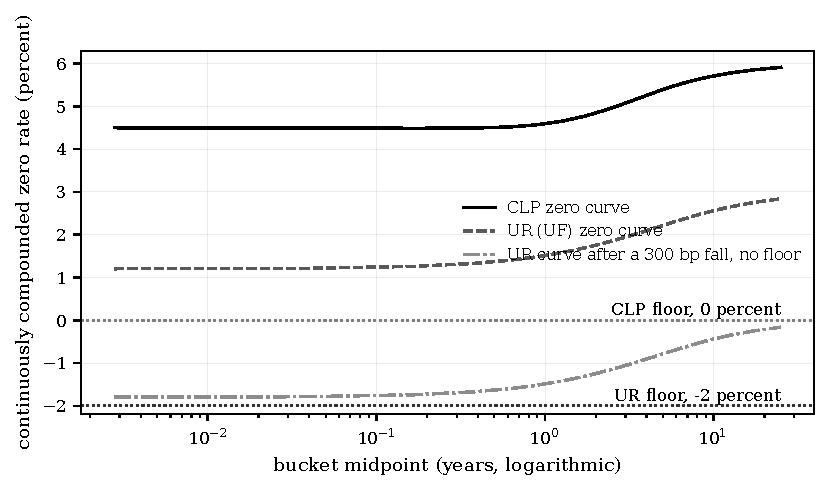
\includegraphics[width=0.78\textwidth]{curves-and-floors}
\caption{The two zero curves fitted by the engine to the Banco Central de Chile yields of 2026-09-03 at the 19 bucket midpoints, the UF curve after a parallel fall of 300 basis points without a floor, and the floors of the two currencies, minus 2 percent for the UF and 0 for the peso; the lowest point of the fallen UF curve is the smallest distance to a floor in the committed documents.}
\label{fig:curves}
\end{figure}

\subsection{The main comparison}
\label{sec:results-main}

Table~\ref{tab:main-results} compares the treatments on 30 books of each of the three variants whose net UF position is 30 percent of level 1 capital. The Annex 1 delta NII is $\mainAnnexNiiLng\pm\mainAnnexNiiLngCi$, $\mainAnnexNiiSht\pm\mainAnnexNiiShtCi$ and $\mainAnnexNiiOff\pm\mainAnnexNiiOffCi$ million pesos, about \mainAnnexNiiTLng{} percent of level 1 capital. The single-currency delta NII is $\mainSingleNiiLng\pm\mainSingleNiiLngCi$, $\mainSingleNiiSht\pm\mainSingleNiiShtCi$ and $\mainSingleNiiOff\pm\mainSingleNiiOffCi$, so the Annex 1 measure is $\mainRatioNiiLng\pm\mainRatioNiiLngCi$, $\mainRatioNiiSht\pm\mainRatioNiiShtCi$ and $\mainRatioNiiOff\pm\mainRatioNiiOffCi$ times larger. These ratios are below those of the committed seed, \repRatioLo{} to \repRatioHi{}: the committed book lies in the upper part of the distribution over books, and the range quoted by the design document is the range of that one book, not of the treatment. The Basel positive-part aggregation gives about three quarters of the Annex 1 income measure (\mainPosOverAnnexNiiLng{}, \mainPosOverAnnexNiiSht{} and \mainPosOverAnnexNiiOff{}), because it has no charge; the earnings gap of the whole book equals the single-currency income measure to the unit in every row, the identity of Section~\ref{sec:method-implementation}. The charge supplies $\mainChargeShareLng\pm\mainChargeShareLngCi$, $\mainChargeShareSht\pm\mainChargeShareShtCi$ and $\mainChargeShareOff\pm\mainChargeShareOffCi$ percent of the Annex 1 income measure.

\begin{table}[htbp]
\centering
\footnotesize
\setlength{\tabcolsep}{3.5pt}
\caption{Main comparison on the three variants whose net UF position is 30 percent of level 1 capital: the delta NII and the delta EVE of the Annex 1 treatment, of the positive-part aggregation of the Basel standard, of the single-currency treatment of the same flows, and of the repricing-gap and duration-gap measures, as the mean and the half-width of the 95 percent Student interval over 30 synthetic books (seeds 1 to 30) on the curves of 2026-09-03; the three right columns divide each mean by the Annex 1 mean.}
\label{tab:main-results}
\begin{tabular}{lrrrrrr}
\toprule
\multicolumn{7}{l}{\textbf{Panel A. Delta NII, CLP million (left: mean $\pm$ 95\% half-width; right: ratio to Annex 1)}} \\
\midrule
Treatment & Long UF & Short UF & Offset on/off & Long UF & Short UF & Offset \\
\midrule
Annex 1 (separate UR) & 11{,}907$\pm$251 & 11{,}772$\pm$252 & 11{,}725$\pm$252 & 1.00 & 1.00 & 1.00 \\
Positive parts (Basel aggregation) & 9{,}039$\pm$230 & 9{,}039$\pm$230 & 9{,}039$\pm$230 & 0.76 & 0.77 & 0.77 \\
Single currency & 2{,}412$\pm$323 & 2{,}143$\pm$325 & 2{,}049$\pm$325 & 0.20 & 0.18 & 0.17 \\
Repricing gap (single currency) & 2{,}412$\pm$323 & 2{,}143$\pm$325 & 2{,}049$\pm$325 & 0.20 & 0.18 & 0.17 \\
\midrule
\multicolumn{7}{l}{\textbf{Panel B. Delta EVE, CLP million (left: mean $\pm$ 95\% half-width; right: ratio to Annex 1)}} \\
\midrule
Treatment & Long UF & Short UF & Offset on/off & Long UF & Short UF & Offset \\
\midrule
Annex 1 (separate UR) & 85{,}061$\pm$1{,}875 & 68{,}605$\pm$2{,}088 & 72{,}044$\pm$1{,}824 & 1.00 & 1.00 & 1.00 \\
Positive parts (Basel aggregation) & 85{,}927$\pm$1{,}810 & 68{,}605$\pm$2{,}088 & 85{,}434$\pm$1{,}792 & 1.01 & 1.00 & 1.19 \\
Single currency & 80{,}186$\pm$1{,}790 & 58{,}057$\pm$1{,}827 & 54{,}645$\pm$1{,}758 & 0.94 & 0.85 & 0.76 \\
Duration gap (single currency) & 91{,}126$\pm$2{,}178 & 64{,}216$\pm$2{,}251 & 59{,}621$\pm$2{,}155 & 1.07 & 0.94 & 0.83 \\
\bottomrule
\end{tabular}
\end{table}


For the value measure the single-currency treatment is $\mainEveShortLng\pm\mainEveShortLngCi$, $\mainEveShortSht\pm\mainEveShortShtCi$ and $\mainEveShortOff\pm\mainEveShortOffCi$ percent below Annex 1. The long UF variant has the smallest shortfall and the offset variant the largest; in the offset variant the two legs move in opposite directions at several scenarios, so that the Basel positive-part aggregation is \mainPosOverAnnexEveOff{} times the Annex 1 measure, the only case in which it differs from it by more than one percent (\mainPosOverAnnexEveLng{} and \mainPosOverAnnexEveSht{} in the other two). The duration gap, a first-order measure of the whole book as one currency, gives \mainGapOverAnnexEveLng{}, \mainGapOverAnnexEveSht{} and \mainGapOverAnnexEveOff{} times the Annex 1 value measure: it is above it for the long UF book and below it for the other two, so a first-order single-currency measure does not have a stable sign against the supervisor's measure. Figure~\ref{fig:main} gives the six variants as a share of level 1 capital. The steepener and floor-exposed variants have a net UF position of 5 percent of level 1 capital and so a small charge; their income ratios, \mainRatioNiiStp{} and \mainRatioNiiFlr{}, are smaller than those of the 30 percent variants, in line with Proposition~\ref{prop:charge}.

\begin{figure}[htbp]
\centering
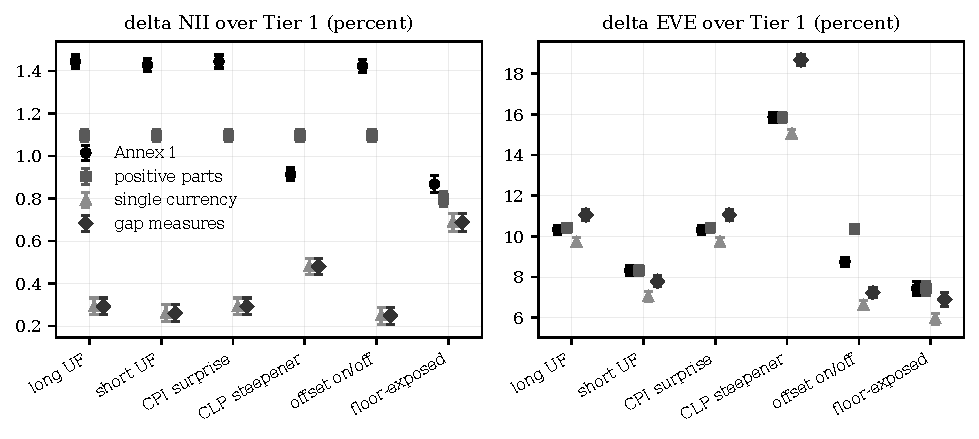
\includegraphics[width=\textwidth]{treatments-over-tier1}
\caption{Delta NII (left) and delta EVE (right) as a percentage of level 1 capital under the Annex 1 treatment, the Basel positive-part aggregation, the single-currency treatment and the repricing-gap and duration-gap measures, for the six variants; points are means over 30 synthetic books and bars are 95 percent half-widths.}
\label{fig:main}
\end{figure}

\subsection{The bound and the first predictions}
\label{sec:results-hypotheses}

H1 holds. In \hOneChecked{} comparisons over six variants, 30 books, eight combinations of curve, sizes and floor, and the two measures, and in \repSandChecked{} further comparisons on the committed seed, there are \hOneViol{} violations of the order $N\le P_{1/2}\le Q$ of Proposition~\ref{prop:pair} (\repSandViol{} on the committed seed). Figure~\ref{fig:pair} draws the three aggregation rules for two legs, one gaining and one losing, from the engine's \texttt{cmf\_pair}: the pair rule lies between the other two and reduces the positive-part sum by at most half of the gain.

\begin{figure}[htbp]
\centering
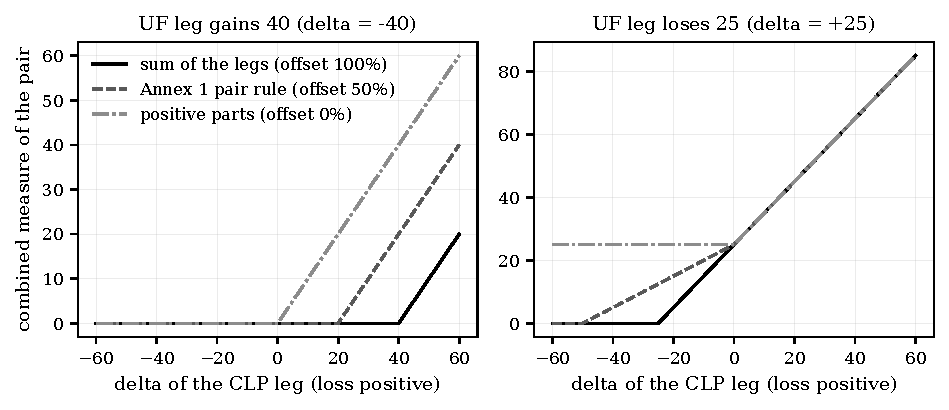
\includegraphics[width=0.92\textwidth]{pair-function}
\caption{The aggregation of the two legs' deltas as a function of the delta of the peso leg, for a UF leg that gains 40 (left) and one that loses 25 (right): the sum of the legs, the pair rule of Annex 1 with a 50 percent offset computed by the engine's cmf\_pair, and the sum of the positive parts used by the Basel standard.}
\label{fig:pair}
\end{figure}

H2 is refuted. In the three variants with a 30 percent position the switch with the largest absolute Shapley value for the delta EVE is the \hTwoTopLng{} in each, not the pair rule (Section~\ref{sec:ablation}). H3 is refuted in one clause: in the CLP steepener variant the Annex 1 delta NII is below the Basel positive-part one in \hThreeSteeperViol{} of 30 books, \mainPosOverAnnexNiiStp{} times larger for the positive parts. Equation~\eqref{eq:charge-condition} gives the reason: the positive part \repPosNiiStp{} exceeds the largest pair \repMaxPairStp{} by more than the charge \repChargeStp{}, because the net UF position is only \repNuStp{} percent of level 1 capital; in the other five variants this clause holds in every book, and the other two clauses of H3 hold in all 180 books. The own curve is also the reason for a result of the theory that the data show directly: discounting the UF assets on the peso curve understates their present value by \repAssetUnderLng{} percent in the committed book, and the UF liabilities of the short UF book by \repLiabUnderSht{} percent, since the discount factor on the peso curve is \dfRatioFive{}, \dfRatioTen{} and \dfRatioLast{} times that on the UF curve at 5.5, 9.5 and 25 years (Figure~\ref{fig:fisher}).

\begin{figure}[htbp]
\centering
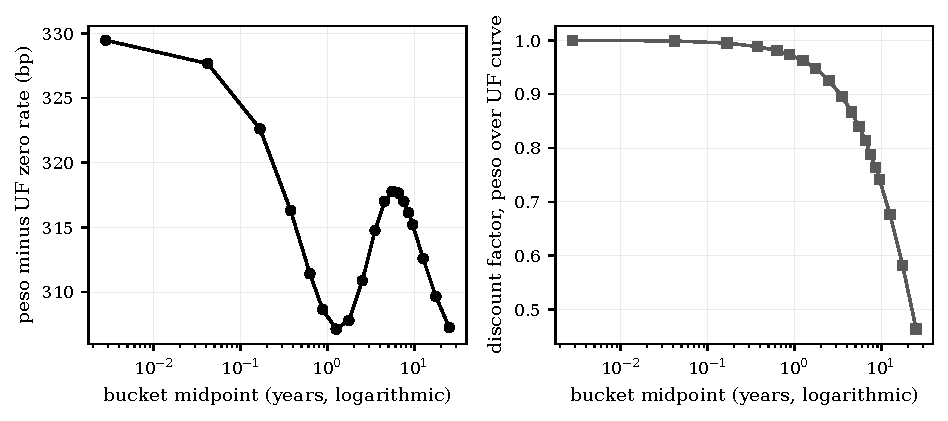
\includegraphics[width=0.92\textwidth]{peso-curve-on-uf-flows}
\caption{The gap between the peso and the UF zero rate (left) and the ratio of the discount factor on the peso curve to the one on the UF curve (right) at the 19 bucket midpoints, from the curves of 2026-09-03; the ratio is the factor by which a peso curve understates the value of an indexed flow.}
\label{fig:fisher}
\end{figure}

\subsection{When the two treatments classify a bank differently}
\label{sec:results-sweep}

Figure~\ref{fig:sweep} and Table~\ref{tab:sweep} give the two measures as a share of level 1 capital against the net UF position of the long UF book, from \sweepLo{} to \sweepHi{} percent; the generator refuses the other \sweepRefused{} of the 31 positions of the grid, those that would need more UF borrowings than the book has. At the position of the committed variants, 30 percent, the Annex 1 income measure is \swThreeAnnexNii{} percent of level 1 capital and the single-currency one \swThreeSingleNii{} percent; the value measures are \swThreeAnnexEve{} and \swThreeSingleEve{} percent. No book is flagged by any treatment up to a position of 50 percent. The Basel positive-part aggregation flags its first books at \sweepPosFlagFirst{} percent, the Annex 1 treatment flags \swTenFlagAnnex{} of 20 books at 100 percent, \swElevenFlagAnnex{} at 110 percent and \swFifteenFlagAnnex{} at 150, while the single-currency treatment flags none up to 110 percent, \swTwelveFlagSingle{} at 120 percent and \swFifteenFlagSingle{} at 150 percent (Figure~\ref{fig:flags}).

\begin{figure}[htbp]
\centering
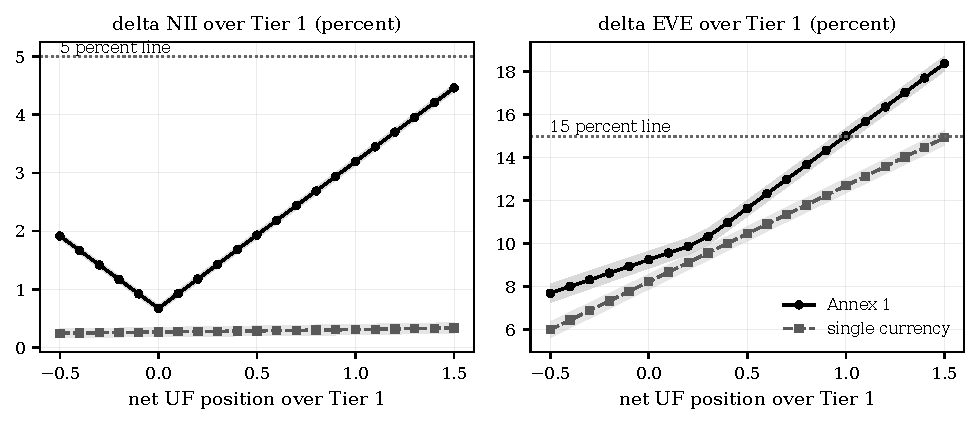
\includegraphics[width=\textwidth]{position-sweep}
\caption{Delta NII (left) and delta EVE (right) as a percentage of level 1 capital against the net UF position, for the Annex 1 and the single-currency treatments, with the 5 and 15 percent prioritisation lines; lines are means over 20 synthetic books and bands are 95 percent intervals.}
\label{fig:sweep}
\end{figure}

\begin{table}[htbp]
\centering
\footnotesize
\setlength{\tabcolsep}{3.5pt}
\caption{The delta NII (NII) and delta EVE (EVE) as a share of level 1 capital under the Annex 1 (A1) and the single-currency (SC) treatments, and the number of the 20 synthetic books (seeds 101 to 120) that Annex 1 (Flag A1), the positive-part aggregation (Flag PP) and the single currency (Flag SC) flag as prioritised under at least one of the three tests of Annex 1, at selected net UF positions of the long UF book (positive: UF assets exceed UF funding).}
\label{tab:sweep}
\begin{tabular}{lrrrrrrr}
\toprule
Net UF / $T_1$ & NII A1 & NII SC & EVE A1 & EVE SC & Flag A1 & Flag PP & Flag SC \\
\midrule
$-$50\% & 1.92\% & 0.25\% & 7.7\% & 6.0\% & 0 & 0 & 0 \\
0\% & 0.67\% & 0.27\% & 9.2\% & 8.2\% & 0 & 0 & 0 \\
30\% & 1.43\% & 0.28\% & 10.3\% & 9.6\% & 0 & 0 & 0 \\
80\% & 2.69\% & 0.30\% & 13.7\% & 11.8\% & 1 & 17 & 0 \\
100\% & 3.19\% & 0.31\% & 15.0\% & 12.7\% & 10 & 20 & 0 \\
110\% & 3.45\% & 0.32\% & 15.7\% & 13.1\% & 17 & 20 & 0 \\
120\% & 3.70\% & 0.32\% & 16.4\% & 13.6\% & 19 & 20 & 1 \\
150\% & 4.46\% & 0.34\% & 18.4\% & 14.9\% & 20 & 20 & 8 \\
\bottomrule
\end{tabular}
\end{table}


H4 holds, narrowly: there are \hFourN{} positions, from \hFourLo{} to \hFourHi{} percent of level 1 capital, at which Annex 1 flags more than half of the books and the single-currency treatment flags none or few. Three qualifications bound the result. The flag is the value test, of 15 percent of level 1 capital, in every case: the income test is never breached by any treatment at any position (the largest mean income measure is \sweepMaxAnnexNii{} percent, below the 5 percent line, and the number of flags of the income tests is \sweepNiiFlagTotal{} and of the margin test \sweepMarginFlagTotal{}), consistent with Proposition~\ref{prop:charge}, which needs a position of \floorBreakNu{} times level 1 capital for the charge alone to breach. The positions are large, a net UF position above the whole of the capital. And the Basel positive-part aggregation flags earlier than either, so that the differing classification is mainly the effect of the pair rule and of the sizes on the value measure and not of the indexation charge.

\begin{figure}[htbp]
\centering
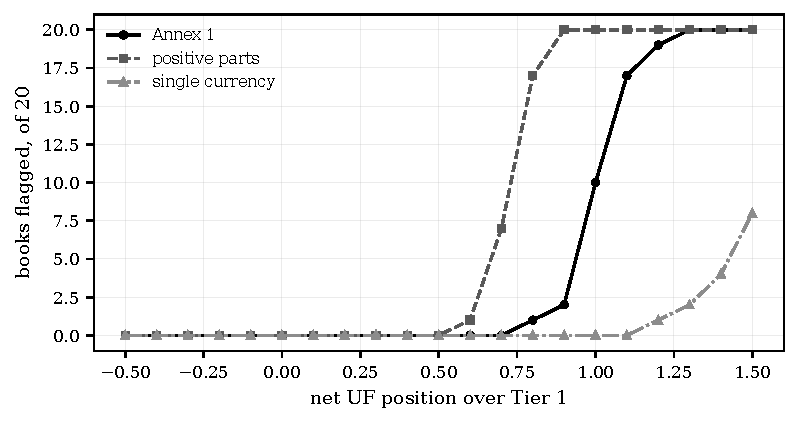
\includegraphics[width=0.78\textwidth]{prioritised-flags}
\caption{The number of the 20 synthetic books flagged as prioritised under at least one of the three tests of Annex 1 against the net UF position, for the Annex 1 treatment, the Basel positive-part aggregation and the single-currency treatment.}
\label{fig:flags}
\end{figure}

\subsection{The floor of the UF made to bind}
\label{sec:results-floors}

On the curves of the valuation date the distance of the lowest post-shock UF rate to its floor is \floorsDistZero{} basis points, so the floor binds nowhere and its effect is not shown by the committed documents. Translating the UF curve down by 25 basis points puts the lowest rate \flTwentyFiveDistLng{} basis points past the floor; the effect on a measure then depends on the book (Table~\ref{tab:floors}, Figure~\ref{fig:floors}). On the delta EVE the floor changes the measure in \floorsEveChanged{} of the comparisons at every translation up to $-300$ basis points, because the scenario that attains the maximum is the parallel-up shock, on which a floor cannot bind. On the delta NII the effect of the floor in the long UF variant is zero up to a translation of 50 basis points, $\flHundredEffLng\pm\flHundredEffLngCi$ at $-100$, $\flTwoHundredEffLng\pm\flTwoHundredEffLngCi$ at $-200$ and $\flThreeHundredEffLng\pm\flThreeHundredEffLngCi$ million pesos at $-300$ basis points, and it is positive: the floor raises the measure, in \flThreeHundredRaiseLng{} of 20 books at $-300$ and in none lowers it. In the floor-exposed variant, whose UF leg is asset-sensitive because 70 percent of its commercial loans float, the floor lowers the measure at small translations (\flFiftyLowerFlr{} of 20 books at $-50$ basis points, mean effect $\flFiftyEffFlr\pm\flFiftyEffFlrCi$) and raises it at large ones (\flThreeHundredRaiseFlr{} of 20 at $-300$, mean $\flThreeHundredEffFlr\pm\flThreeHundredEffFlrCi$).

\begin{table}[htbp]
\centering
\footnotesize
\setlength{\tabcolsep}{3.5pt}
\caption{The UR floor of minus 2 percent made to bind by translating the fitted UF zero curve down: the mean distance of the lowest post-shock UR rate to the floor (negative once it binds), the Annex 1 delta NII without any floor and with the floor, the effect of the floor with its 95 percent half-width, and the number of the 20 books (seeds 201 to 220) in which the floor raises or lowers the measure, for two variants.}
\label{tab:floors}
\begin{tabular}{lrrrrrr}
\toprule
\multicolumn{7}{l}{\textbf{Panel A. Delta NII, long uf variant, CLP million}} \\
\midrule
Shift (bp) & Dist. (bp) & No floor & Floor & Effect & Raised & Lowered \\
\midrule
+0 & 20.5 & 11{,}711 & 11{,}711 & 0$\pm$0 & 0 & 0 \\
$-$25 & -4.5 & 11{,}711 & 11{,}711 & 0$\pm$0 & 0 & 0 \\
$-$50 & -29.5 & 11{,}711 & 11{,}711 & 0$\pm$0 & 0 & 0 \\
$-$100 & -79.5 & 11{,}711 & 11{,}719 & 8$\pm$16 & 1 & 0 \\
$-$200 & -179.5 & 11{,}711 & 11{,}832 & 120$\pm$156 & 6 & 0 \\
$-$300 & -279.5 & 11{,}711 & 12{,}392 & 681$\pm$404 & 11 & 0 \\
\midrule
\multicolumn{7}{l}{\textbf{Panel B. Delta NII, floor-exposed variant, CLP million}} \\
\midrule
Shift (bp) & Dist. (bp) & No floor & Floor & Effect & Raised & Lowered \\
\midrule
+0 & 20.5 & 7{,}041 & 7{,}041 & 0$\pm$0 & 0 & 0 \\
$-$25 & -4.5 & 7{,}041 & 7{,}041 & 0$\pm$0 & 0 & 0 \\
$-$50 & -29.5 & 7{,}041 & 7{,}022 & $-$19$\pm$15 & 2 & 18 \\
$-$100 & -79.5 & 7{,}041 & 7{,}100 & 58$\pm$40 & 15 & 5 \\
$-$200 & -179.5 & 7{,}041 & 7{,}256 & 215$\pm$90 & 16 & 4 \\
$-$300 & -279.5 & 7{,}041 & 7{,}413 & 372$\pm$140 & 17 & 3 \\
\bottomrule
\end{tabular}
\end{table}


\begin{figure}[htbp]
\centering
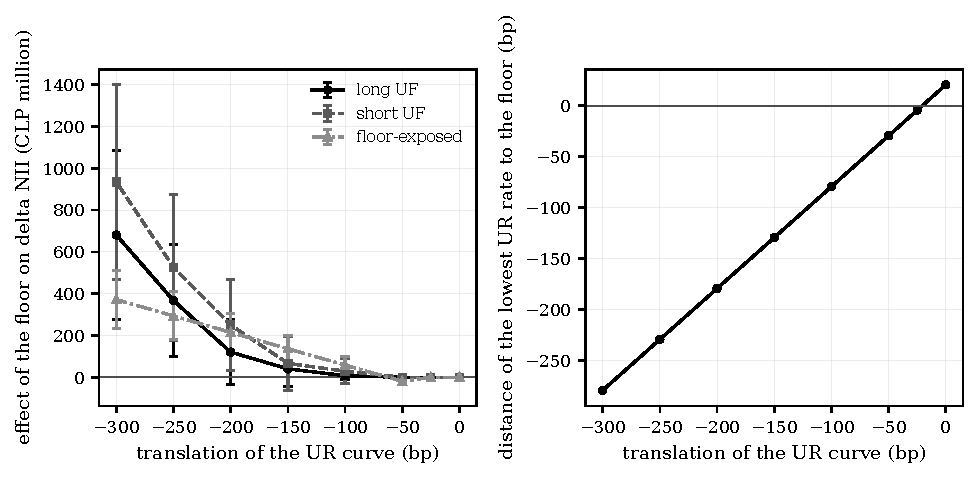
\includegraphics[width=\textwidth]{floor-effect}
\caption{Effect of the UF floor on the Annex 1 delta NII against the translation of the UF curve for three variants (left; means over 20 books with 95 percent intervals) and the distance of the lowest post-shock UF rate to the floor for the long UF variant (right).}
\label{fig:floors}
\end{figure}

H5 is refuted: \floorsRaise{} of \floorsTotal{} comparisons of the two measures over six variants, eight translations and 20 books show a measure with the floor above the measure without it, by up to \floorsMaxInc{} million pesos. The sign follows Proposition~\ref{prop:floor}: a liability-sensitive UF leg, as in the long UF, short UF and offset variants, has a gain in the falling scenario that the floor reduces, and the pair rule then offsets less of it against the peso loss. Across the five variants other than the floor-exposed one the floor lowers the measure in \floorsLowerOthers{} books, and in the floor-exposed one it lowers it in \floorsLowerTotalFlr{} and raises it in \floorsRaiseTotalFlr{} of the 160 book and translation pairs.


\section{Ablation}
\label{sec:ablation}
\subsection{The Shapley values of the five switches}
\label{sec:ablation-shapley}

Table~\ref{tab:shapley} gives the exact Shapley value of each switch for the two measures in the three variants whose net UF position is 30 percent of level 1 capital, and Figure~\ref{fig:shapley} draws them. For the income measure the picture is that of the theory. The charge has the value $\mainShapNiiChargeLng\pm\mainShapNiiChargeLngCi$ million pesos in each of the three variants, the constant $\kappa|\PNUR|$ of Proposition~\ref{prop:shapley} with no interval because it does not vary across books. The own sizes switch has the value $\mainShapNiiSizesLng\pm\mainShapNiiSizesLngCi$, the dummy of the same proposition. The pair rule has $\mainShapNiiPairLng\pm\mainShapNiiPairLngCi$, $\mainShapNiiPairSht\pm\mainShapNiiPairShtCi$ and $\mainShapNiiPairOff\pm\mainShapNiiPairOffCi$, a little more than half of the charge, and the own curve and the own floor are small, $\mainShapNiiCurveLng\pm\mainShapNiiCurveLngCi$ and $\mainShapNiiFloorLng\pm\mainShapNiiFloorLngCi$ in the long UF variant, because they act only when the floor of zero binds on the low short rates of the UF curve. The income gap between the two treatments is therefore carried by the aggregation and the charge, in the proportion of about one to two.

\begin{table}[htbp]
\centering
\footnotesize
\setlength{\tabcolsep}{3.5pt}
\caption{Exact Shapley value of each of the five switches that turn the single-currency treatment of the UF leg into the Annex 1 treatment, for the three variants with a net UF position of 30 percent of level 1 capital, as the mean and the 95 percent half-width over 30 synthetic books; each panel's last row is the Annex 1 measure minus the single-currency measure, which the five values add up to.}
\label{tab:shapley}
\begin{tabular}{lrrr}
\toprule
\multicolumn{4}{l}{\textbf{Panel A. Delta EVE, CLP million}} \\
\midrule
Switch turned on & Long UF & Short UF & Offset on/off \\
\midrule
Own curve & 32{,}767$\pm$956 & 18{,}927$\pm$1{,}029 & 32{,}724$\pm$976 \\
Own shock sizes & $-$28{,}757$\pm$568 & $-$8{,}379$\pm$597 & $-$28{,}671$\pm$628 \\
Own floor & 0$\pm$0 & 0$\pm$0 & 0$\pm$0 \\
Pair rule with offset & 866$\pm$367 & 0$\pm$0 & 13{,}346$\pm$468 \\
Indexation charge & 0$\pm$0 & 0$\pm$0 & 0$\pm$0 \\
Sum: Annex 1 minus single currency & 4{,}875 & 10{,}548 & 17{,}399 \\
\midrule
\multicolumn{4}{l}{\textbf{Panel B. Delta NII, CLP million}} \\
\midrule
Switch turned on & Long UF & Short UF & Offset on/off \\
\midrule
Own curve & 283$\pm$139 & 421$\pm$163 & 475$\pm$172 \\
Own shock sizes & 0$\pm$0 & 0$\pm$0 & 0$\pm$0 \\
Own floor & $-$172$\pm$101 & $-$257$\pm$122 & $-$295$\pm$130 \\
Pair rule with offset & 3{,}202$\pm$99 & 3{,}283$\pm$97 & 3{,}315$\pm$96 \\
Indexation charge & 6{,}182$\pm$0 & 6{,}182$\pm$0 & 6{,}182$\pm$0 \\
Sum: Annex 1 minus single currency & 9{,}495 & 9{,}630 & 9{,}677 \\
\bottomrule
\end{tabular}
\end{table}


For the value measure the picture is different, and it is the result that refutes H2. The own curve has the value $\mainShapEveCurveLng\pm\mainShapEveCurveLngCi$, $\mainShapEveCurveSht\pm\mainShapEveCurveShtCi$ and $\mainShapEveCurveOff\pm\mainShapEveCurveOffCi$ million pesos in the three variants, and the own sizes $\mainShapEveSizesLng\pm\mainShapEveSizesLngCi$, $\mainShapEveSizesSht\pm\mainShapEveSizesShtCi$ and $\mainShapEveSizesOff\pm\mainShapEveSizesOffCi$, with the opposite sign. The two nearly cancel in the long UF and the offset variants, so that the difference of the two measures, \repAnnexEveLng{} against \repSingleEveLng{} million pesos at the committed seed in the long UF variant, is a small remainder of two large terms. The pair rule has $\mainShapEvePairLng\pm\mainShapEvePairLngCi$, $\mainShapEvePairSht\pm\mainShapEvePairShtCi$ and $\mainShapEvePairOff\pm\mainShapEvePairOffCi$: it matters for the value measure only in the offset variant, whose peso bonds are twice as long and whose legs move in opposite directions at several scenarios, and not where the argmax scenario is the parallel-up shock at which both legs lose. The floor and the charge are zero, the floor because no floor binds in a value scenario that attains the maximum, the charge by construction.

\begin{figure}[htbp]
\centering
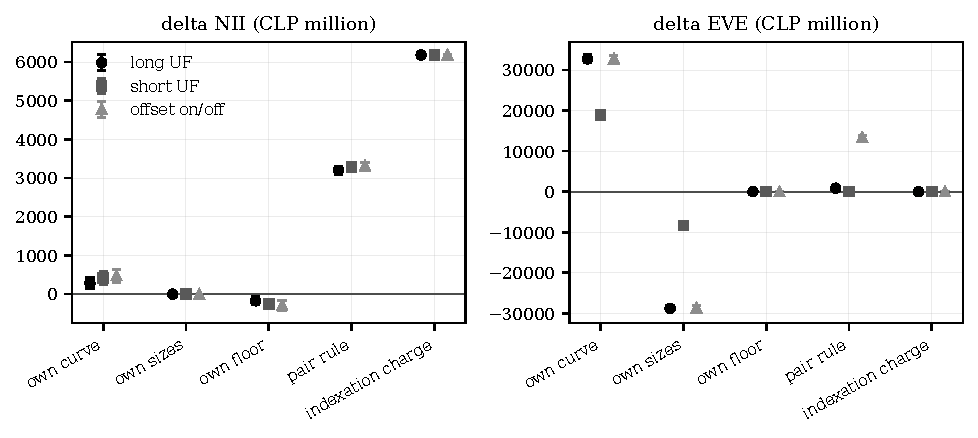
\includegraphics[width=\textwidth]{shapley-values}
\caption{Exact Shapley value of each of the five switches for the delta NII (left) and the delta EVE (right) in the three variants with a 30 percent net UF position, as means over 30 synthetic books with 95 percent intervals.}
\label{fig:shapley}
\end{figure}

\subsection{One at a time, and the interaction between the switches}
\label{sec:ablation-oat}

Table~\ref{tab:ablation} gives, for the long UF variant, the change of each measure when a switch is turned off in the Annex 1 treatment, the change when it alone is turned on in the single-currency treatment, and the Shapley value. For the value measure, turning the own curve on alone adds $\mainAoiEveCurveLng$ million pesos, turning it off in Annex 1 removes $\mainLooEveCurveLng$ and the Shapley value is $\mainShapEveCurveLng$: the three differ by about 20 percent, which is the interaction of the curve with the sizes, since the first-order weight $w_k$ of Equation~\eqref{eq:weight} depends on both. The same holds for the sizes, $\mainAoiEveSizesLng$, $\mainLooEveSizesLng$ and $\mainShapEveSizesLng$. For the income measure the three quantities coincide for the charge ($\mainAoiNiiChargeLng$, $\mainLooNiiChargeLng$, $\mainShapNiiChargeLng$) and for the pair rule to within the width of the interval ($\mainAoiNiiPairLng$, $\mainLooNiiPairLng$, $\mainShapNiiPairLng$): the additive switches do not interact, which is what makes the attribution of the income gap unambiguous. The own curve has a first-order effect of $\mainAoiNiiCurveLng$ when it acts alone and none when it is turned off in Annex 1, an interaction with the floor: with the peso floor of zero the fall of 300 basis points takes the low UF rates below zero and the floor binds, which changes the income measure, and with the floor of minus two percent it does not bind, so the curve then changes nothing (Proposition~\ref{prop:floor}). No other switch changes sign across the three quantities.

\begin{table}[htbp]
\centering
\footnotesize
\setlength{\tabcolsep}{3.5pt}
\caption{One-at-a-time ablation on the long UF variant, as the mean and the 95 percent half-width over 30 books: the change of the measure when a switch is turned off in Annex 1 (the first column is the measure without the switch minus the Annex 1 measure) and when it alone is turned on in the single-currency treatment, beside the Shapley value that averages the change over every order of the five switches.}
\label{tab:ablation}
\begin{tabular}{lrrr}
\toprule
\multicolumn{4}{l}{\textbf{Panel A. Delta EVE, long UF variant, CLP million}} \\
\midrule
Switch & Annex 1 without it & Single currency with it & Shapley value \\
\midrule
Own curve & $-$27{,}228$\pm$800 & 38{,}306$\pm$1{,}112 & 32{,}767$\pm$956 \\
Own shock sizes & 34{,}296$\pm$704 & $-$23{,}218$\pm$446 & $-$28{,}757$\pm$568 \\
Own floor & 0$\pm$0 & 0$\pm$0 & 0$\pm$0 \\
Pair rule with offset & $-$866$\pm$367 & 866$\pm$367 & 866$\pm$367 \\
Indexation charge & 0$\pm$0 & 0$\pm$0 & 0$\pm$0 \\
\midrule
\multicolumn{4}{l}{\textbf{Panel B. Delta NII, long UF variant, CLP million}} \\
\midrule
Switch & Annex 1 without it & Single currency with it & Shapley value \\
\midrule
Own curve & 0$\pm$0 & 787$\pm$357 & 283$\pm$139 \\
Own shock sizes & 0$\pm$0 & 0$\pm$0 & 0$\pm$0 \\
Own floor & 122$\pm$134 & 0$\pm$0 & $-$172$\pm$101 \\
Pair rule with offset & $-$3{,}313$\pm$125 & 3{,}313$\pm$125 & 3{,}202$\pm$99 \\
Indexation charge & $-$6{,}182$\pm$0 & 6{,}182$\pm$0 & 6{,}182$\pm$0 \\
\bottomrule
\end{tabular}
\end{table}


Two conclusions follow for the use of the measure. A reader who wants to know what the separate treatment adds to the income measure can read it from two numbers, the charge and the offset, and the sum is stable across books. A reader who wants the same for the value measure cannot read it from the sum: the gap between the two treatments is small because a real curve that raises the sensitivity of the UF flows and a smaller table of sizes that lowers it nearly offset each other, and a change in either input of the supervisor's text, a recalibrated size table for example, would move the gap by tens of thousands of millions of pesos without any change in the treatment of the UF as a currency.


\section{Discussion}
\label{sec:discussion}
The results say that the separate treatment of the UF changes the Annex 1 measures in two different ways, and that the two ways have different causes. The income measure differs from its single-currency counterpart through two additive terms that need no market input: the charge, which is a fixed fraction of the position, and the offset that is only half of what a netting would give. Both are rules of the text and not estimates, and the proportion of about one to two in which the pair rule and the charge carry the gap is stable across books (Table~\ref{tab:shapley}). The value measure differs through two inputs that depend on the market and on the supervisor's calibration, the real curve and the table of sizes, whose effects nearly cancel on the book studied. The sign of each is as Proposition~\ref{prop:curve} says, a large positive effect of the real curve on the sensitivity of the UF flows against a negative one of the smaller sizes, but the near cancellation is a property of the book and of the two curves of the valuation date, not of the treatment: the weight $w_k$ crosses one between \tStarLo{} and \tStarHi{} years, and a book whose UF flows lay beyond that horizon would have the single-currency treatment below Annex 1 for the value measure by more than the book studied, while a book of short flows would have it above.

The failures are informative. H2 failed because it expected the aggregation rule, the visible feature of the text, to carry the value measure; the data say the inputs carry it. H3 failed in one clause because the charge is a constant that does not scale with the size of the offset, so that for a small net UF position the Annex 1 income measure can fall below the Basel positive-part aggregation, a condition that Equation~\eqref{eq:charge-condition} states exactly and that makes the Basel aggregation, in books with a large offset and a small position, the more conservative of the two. H5 failed because a floor, which is natural to read as a limit on the shock, interacts with a pair rule that offsets gains: reducing the gain of one leg reduces what is offset, and the measure rises. A supervisor or a bank that tests the floor by asking whether the measure falls when it is imposed would be misled in the books that Table~\ref{tab:floors} shows.

The practical reading depends on the audience. For a bank, the charge is a lower bound on the income measure that no hedge of the rate risk removes, and it is 2.5 percent of the position, so that a net UF position of 30 percent of level 1 capital uses 0.75 percent of the 5 percent line (\repChargeOverTier{} percent in the short UF variant). The test of the income measure cannot be breached by the charge alone short of a position of \floorBreakNu{} times capital, so for a bank with a UF position of ordinary size the measure that classifies it is the value measure, which the near cancellation of the two inputs leaves close to what a single-currency calculation gives (the single-currency value measure is $\mainSingleOverAnnexEveLng$ of Annex 1 in the long UF variant). For a validator of such a bank's model, the decomposition gives a way to test an implementation: the dummy and the charge of Proposition~\ref{prop:shapley} are exact, the sandwich of Proposition~\ref{prop:pair} is an inequality that any implementation of the pair rule must satisfy, and a defect in either shows at once.

The result of the sweep, that the two treatments classify more than half of the books differently only at positions of \sweepMajLo{} to \sweepMajHi{} percent of level 1 capital, the top of the range tested, and single books from \sweepFirstDiff{} percent, has a second reading. A treatment that differs by a factor of about five in an income measure and by \mainEveShortLo{} to \mainEveShortHi{} percent in a value measure, and yet changes the classification of no book at the positions of 30 percent and below, is a difference that is invisible to the thresholds and visible in the limits. The board limits of the text are set as percentages of the margin and of level 1 capital, and a limit on the income measure at a fixed share of the margin would be reached at very different positions under the two treatments. The classification is what the supervisor uses, so the factor measures a difference in the measure and not in the supervisory outcome at the positions studied; the paper therefore reports what each component adds to the measures and goes no further.


\section{Limitations}
\label{sec:limitations}
\paragraph{Internal validity.}
The measures are computed by one engine and the result is a function of the engine's reading of the supervisor's text. The reading was checked against the text of Annex 1 for the sizes, the floors, the pair rule, the charge, the grid and the thresholds, and the contract tests of the engine reproduce its golden values; there is no second implementation of Annex 1 to reconcile with, so a defect common to the text's reading and the engine would be invisible. The reading of the floor provision that keeps a pre-shock rate below the floor is settled by the plural of the text (``estos pisos'') but is still a reading. The comparison across seeds measures the variation of the synthetic balance sheet; it does not measure the uncertainty of the curve, which is one fit of one day, with four points per curve and a root-mean-square error of \rmseClp{} and \rmseUr{} basis points, and with a policy rate in place of a missing peso yield. The yields are read as semiannual bond-equivalent par yields, which has not been checked against the central bank's methodology note.

\paragraph{External validity.}
Banco Andino is synthetic. Its totals are calibrated to the banking system, but the UF share of each portfolio, the repricing profile of each item, the deposit split and every behavioural parameter are assumptions, so the proportions of the Shapley values describe the treatment on this book and not any bank. The cancellation of the own curve and the own sizes in the value measure depends on where the UF flows lie in the grid; a bank with other maturities would have other weights. The net UF positions at which the two treatments classify more than half of the books differently, \sweepMajLo{} to \sweepMajHi{} percent of level 1 capital, are at or above the whole capital of the bank, and \sweepGridHi{} percent is the top of the range tested, so the sweep does not show where the difference ends; single books differ from \sweepFirstDiff{} percent. It is not known whether any Chilean bank holds a position of that size, which the aggregates published by the supervisor do not state. The curves are those of one day, September 2026; periods of negative real rates, in which the floor of minus two percent was designed to matter, are not in the raw files, and the floor experiment replaces them by a translation of the fitted curve, which is a what-if and not a history.

\paragraph{Construct validity.}
The paper measures a rule, not an exposure. The Annex 1 measure is a standardised supervisory number; it assumes a run-off balance for the value measure and a constant balance for the income measure, ignores the optionality that the text treats separately, and applies one set of behavioural factors. A difference between the Annex 1 and the single-currency measures is not a difference in the risk of a bank. The single-currency treatment is a counterfactual that a bank aware of indexed units would not use, and the comparison shows what the separate treatment adds to a number; it does not show that a bank that used the counterfactual would misjudge its risk. The indexation charge is read as a stress of 2.5 percentage points in either direction, and the paper does not model the process of inflation or the one-month lag of the UF accrual. The attribution by the Shapley value depends on the choice of five switches; a different partition of the treatment, the curve and the sizes as one switch for example, would give other values, and the paper does not claim that the five are the only decomposition.

\paragraph{Scope.}
The measurement is for a bank whose significant currencies are the peso and the UR, and the aggregation across further currencies is not studied. The option treatment of the text is not implemented. The hedges and the dynamic balance sheet are outside the standardised measures. The statements about the absence of a public implementation of Annex 1 and of a published decomposition are limited to the search behind this work.


\section{Reproducibility}
\label{sec:reproducibility}
The code, the data and the commands are in the repository of the product, \url{https://github.com/fsantibanezleal/CAOS_Contraste}, in the folder \url{manuscripts/uf-as-its-own-currency-in-irrbb}. The engine is \texttt{riskvalidation} 1.1.0 and the committed C15 documents are in \texttt{data/derived/C15}. The raw Banco Central de Chile files are in the data root of the device (\texttt{raw/bcch-f022} under the folder named by the environment variable \texttt{CONTRASTE\_DATA}); each is checked against its provenance record before use and no experiment queries the central bank. From the root of the repository, in the order given, the scripts \texttt{experiments/exp\_reproduce.py}, \texttt{exp\_main.py}, \texttt{exp\_sweep.py} and \texttt{exp\_floors.py}, run with \texttt{python}, write the four JSON outputs, \texttt{figures/make\_figures.py} writes the eight figures and \texttt{tables/make\_tables.py} writes the ten tables and the macros of every number quoted in the text. The experiments are deterministic given the seeds stated in Section~\ref{sec:design-protocol}, and the module \texttt{uf\_core} builds nothing that the engine or the generator of the case does not. The measured run times are \repSeconds{} seconds for the reproduction, \mainSeconds{} for the main comparison and its decomposition, \sweepSeconds{} for the sweep and \floorsSeconds{} for the floor experiment, \totalSeconds{} seconds in all on one workstation, written by the scripts into the JSON outputs.


\section{Conclusions}
\label{sec:conclusions}
Treating the UF as its own currency in the standardised measures changes the income measure far more than the value measure, and for different reasons. On the committed book the single-currency treatment of the same flows gives an income measure \repRatioLo{} to \repRatioHi{} times smaller and a value measure \repEveShortLo{} to \repEveShortHi{} percent smaller in the three variants with a net UF position of 30 percent of level 1 capital; over 30 books the income ratios are $\mainRatioNiiLng\pm\mainRatioNiiLngCi$, $\mainRatioNiiSht\pm\mainRatioNiiShtCi$ and $\mainRatioNiiOff\pm\mainRatioNiiOffCi$ and the value shortfalls $\mainEveShortLng\pm\mainEveShortLngCi$, $\mainEveShortSht\pm\mainEveShortShtCi$ and $\mainEveShortOff\pm\mainEveShortOffCi$ percent. The exact Shapley decomposition attributes the income gap to the indexation charge, which is the constant $\kappa|\PNUR|$, and to the pair rule, in a proportion of about two to one, and the value gap to the own curve and the own sizes, which nearly cancel, with the pair rule small except where the two legs move in opposite directions.

Two of the predictions and one further statement were refuted in whole or in part, and the refutations are results. The pair rule does not dominate the value measure. The Annex 1 income measure does not always exceed the Basel positive-part aggregation: it falls below it when the charge is smaller than the offset reduction, as Equation~\eqref{eq:charge-condition} states. A binding UF floor can raise a measure, in \floorsRaise{} of \floorsTotal{} comparisons after the curve is translated down, because it reduces the gain that the pair rule offsets. The bound that places the pair rule between the sum of the legs and the positive parts held in every one of the \hOneChecked{} comparisons, and the two classifications differ only at net UF positions of \hFourLo{} to \hFourHi{} percent of level 1 capital, through the value test.

The next steps are to run the decomposition on the flows of a real bank where one is available, to replace the translation of the curve by historical periods of negative real rates when their yields are in the raw data, to obtain a second implementation of Annex 1 to reconcile with, and to extend the five switches to the option treatment and to a third currency. The numbers are those of a synthetic bank over the curves of one day.


\bibliographystyle{plainnat}
\bibliography{references}

\end{document}
